\documentclass{report}

% packages
\usepackage[utf8]{inputenc}
\usepackage[ruled,vlined,linesnumbered,noend]{algorithm2e}
\usepackage{amsthm}
\usepackage{amsmath}
\usepackage{amssymb}
\usepackage{enumerate}
\usepackage{dsfont}
\usepackage{graphicx}
\usepackage[margin=1.4in]{geometry}
\usepackage{calrsfs}
\usepackage[nottoc,notlot,notlof]{tocbibind}
\usepackage[dvipsnames]{xcolor}

\usepackage{sectsty}
\chapterfont{\color{RoyalBlue}}  % sets colour of chapters
\sectionfont{\color{RoyalBlue}}  % sets colour of sections
\subsectionfont{\color{RoyalBlue}}  % sets colour of sections

\usepackage{hyperref}
\hypersetup{
    colorlinks=true,
    linkcolor=BrickRed,
    filecolor=magenta,      
    urlcolor=cyan,
    citecolor=OliveGreen,
}

% Theorem env.
\newtheorem{theorem}{Theorem}[section]
\newtheorem{lemma}[theorem]{Lemma}
\newtheorem{conjecture}[theorem]{Conjecture}
\newtheorem{corollary}[theorem]{Corollary}
\newtheorem{proposition}[theorem]{Proposition}
\newtheorem{definition}[theorem]{Definition}
\newtheorem{invariant}[theorem]{Invariant}
\newtheorem{remark}[theorem]{Remark}

% Starred theorem env.
\newtheorem{theorem*}{Theorem*}[section]
\newtheorem{lemma*}[theorem]{Lemma*}
\newtheorem{corollary*}[theorem]{Corollary*}
\newtheorem{proposition*}[theorem]{Proposition*}

% new commands
\DeclareMathAlphabet{\pazocal}{OMS}{zplm}{m}{n}
\DeclareMathOperator*{\polylog}{polylog}
\newcommand{\norm}[1]{\left\lVert#1\right\rVert}

% title and author
\title{\large{- Discrete Mathematics Project -} \\ \LARGE{Incremental Cycle Detection and Topological Ordering} \\ (DRAFT 1)}
\author{\Large{Martin Costa}\footnote{id : u1804635, email : Martin.Costa@warwick.ac.uk} \\
[1.5cm]Supervised by \\
{Prof. Sayan Bhattacharya}}
\date{\vspace*{8cm}October 2020}

% begin the document
\begin{document}

% create the title
\maketitle

\tableofcontents

%%%%____%%%% CHAPTER 1 : INTRODUCTION %%%%____%%%% 
\chapter{Introduction}\label{chapter1}

% OVERVIEW
In this chapter I will start off by introducing to the problems of \textit{incremental cycle detection} and \textit{incremental topological ordering}, followed by formal descriptions of the problems as well as some notation that will be helpful. Finally, I will give an overview of what I will be covering in the different sections of this report.

% SECTION 1.1
\section{Incremental Cycle Detection}

Cycle detection in directed graphs is one of the classic problems studied in algorithmic graph theory. The problem is simple, given some directed graph $G$, return whether or not $G$ is acyclic. The solution is straightforward and can be computed in $\pazocal O(n+m)$ time, where $n$ is the number of \textit{nodes} in $G$ and $m$ is the number of \textit{edges} in $G$.

In this project I will be considering a dynamic version of this problem, where we are given a graph that initially has no edges (and hence no cycles) which is updated over time by a sequence of edge insertions. After each edge is inserted, we must return whether or not the updated graph is acyclic. This problem is referred to as \textit{incremental cycle detection}.

% SECTION 1.1
\section{Incremental Topological Ordering}

We can can come up with a dynamic version of the \textit{topological ordering} problem in a similar way, where we are given a graph that initially has no edges (and hence admits a topological ordering) which is updated over time by a sequence of edge insertions. After each edge is inserted, we must return a topological ordering of the updated graph, and a warning if the updated graph does not admit a topological ordering. This problem is referred to as \textit{incremental topological ordering}.

The fact that a graph $G$ admits a topological ordering of it's nodes if and only if $G$ is a \textit{directed acyclic graph} (DAG) is also one of the standard results in algorithmic graph theory. In fact, the most well known algorithm for cycle detection in directed graphs relies on this equivalence, and determines the presence of a cycle in $G$ by checking whether or not $G$ admits a topological ordering. The problem of cycle detection can be reduced to the problem of topological ordering, as long as we ensure that when no topological ordering exists we return the appropriate warning instead of continuing as normal.

It should then be no surprise that the problems of incremental cycle detection and incremental topological ordering are also deeply connected, and that incremental cycle detection can also be reduced to incremental topological ordering, with the same caveat as before. Because of this, every well known algorithm for incremental cycle detection relies on an algorithm for incremental topological ordering.

% SECTION 1.3
\section{Notation}\label{notation}

Let $G=(V,E)$ be a directed graph with $n=\vert V \vert$ and $m=\vert E \vert$. Given some countable set $S$, denote by $\mathcal{S}_{S}$ the space of all sequences over $S$ where each element of $S$ appears exactly once. Given some $\pazocal S \in \mathcal S_S$ we denote the $i^{th}$ element in the sequence by $\pazocal S_i$, i.e. $\pazocal S = (\pazocal S_1, \pazocal S_2,...)$. Notice that $\mathcal S_E$ is the set of all possible sequences of edge insertions that can be made to construct the graph $G$, we will call the elements of $\mathcal S_E$ the \textit{insertion sequences} of $G$. Define a correspondence, $\sim$, between \textit{total orderings of $V$} and elements of $\mathcal S_V$ such that given some total ordering of $V$, $\prec$, and some $(u_1,...,u_n) \in \mathcal S_V$, we have $\prec \: \sim \pazocal (u_1,...,u_n)$ if and only if $u_1 \prec ... \prec u_n$. This correspondence clearly gives us a bijection between the total orderings of $V$ and elements of $\mathcal S_V$. For the purposes of this report we shall consider a total ordering and its corresponding sequence to be essentially the same, and shall abuse this notation later on. We call the elements of $\mathcal S_V$ the \textit{orderings} of $G$. Given some $\pazocal E \in \mathcal S_E$, denote by $G^{\pazocal E}_t$ the graph $(V, \{\pazocal E_1,..., \pazocal E_t \})$, i.e. the graph $(V, \varnothing)$ after inserting the first $t$ edges in $\pazocal E$. When considering some incremental topological ordering algorithm, $\pazocal A$, some insertion sequence $\pazocal E$ and some ordering $\prec$, we frequently denote by $\prec_t$ the topological ordering computed by $\pazocal A$ starting with the initial ordering $\prec$ after the insertion of the first $t$ edges from $\pazocal E$.

% SECTION 1.4
\section{Overview}

This report will be split up into 6 further chapters. In the next chapter I shall cover the main results on this topic and give an overview of the relevant literature. The rest of the report will cover various original results and ideas that came out of this project, including a framework for designing divide and conquer algorithms for incremental topological ordering and a framework leading to significant progress and partial results for currently open conjectures. The following gives a brief overview of the content contained in each chapter.

\begin{enumerate}[-]

    \item \textbf{Chapter \ref{chapter2}.} A survey of the current state of the problem. Such as going over how the problem is \textit{well understood} for dense graphs but not for sparse graphs, and giving some of the more important results in the area.
    
    \item \textbf{Chapter \ref{chapter3}.} An introduction to the \textit{recourse} of an algorithm (an important metric on incremental topological ordering algorithms). Definitions of the \textit{simple one-way search algorithm} $\pazocal A_1$ and the \textit{simple greedy two-way search algorithm} $\pazocal A_2$; accompanied by an introduction to the random-order model and the conjectures that $\pazocal A_1$ and $\pazocal A_2$ have low recourse under random order arrival, as well as the experimental evidence to support this.
    
    \item \textbf{Chapter \ref{chapter4}.} A description of my framework for divide and conquer incremental topological ordering algorithms. The construction of an algorithm using this framework accompanied by experimental results. 
    
    \item \textbf{Chapter \ref{chapter5}.} A proof that $\pazocal A_2$ obtains $\pazocal O(n \sqrt m)$ recourse under adversarial arrival and the construction of sparse graphs (with corresponding insertion sequences and initial orderings) that yield $\Omega(n \sqrt m)$ recourse on all local algorithms under adversarial arrival; followed by a detailed analysis that shows how the latter does not hold under random-order arrival.
    
    \item \textbf{Chapter \ref{chapter6}.} The construction of a framework using the properties of $\pazocal A_1$ combined with my notion of \textit{activation sequences}, followed by a proof (resulting from this framework) that the expected total recourse of trees under adversarial arrival is $\pazocal O(n \log n)$ with expectation taken over initial orderings.
    
    \item \textbf{Chapter \ref{chapter7}.} An extension of the framework from the previous chapter which shows how the proof of a statement resulting naturally from this framework yields the solution to a currently open problem.
\end{enumerate}

%%%%____%%%% CHAPTER 2 : LITERATURE REVIEW %%%%____%%%%
\chapter{Survey}\label{chapter2}

This chapter starts off with a more detailed introduction to incremental cycle detection and topological ordering, and then goes on to survey the more important and relevant results on the topic, as well as a brief overview of some of the literature which I read throughout the course of the project.

\section{Formal Definition}

Using the notation given in section $\ref{notation}$, the problem of incremental cycle detection is defined formally as follows. Let $G=(V,E)$ be a directed graph, and let $\pazocal E$ be some insertion sequence of $G$. We are given the graph $G^{\pazocal E}_{0} = (V, \varnothing)$ which contains no edges. Subsequently, there are $m$ time-steps. At the $t^{th}$ time step, the edge $\pazocal E_t$ is inserted into the graph, giving us the updated graph $G^{\pazocal E}_t$, we refer to this as an \textit{update} or an \textit{edge insertion}. After each update we must return whether the updated graph contains a cycle. The time taken to report whether the updated graph contains a cycle after the edge insertion is called the \textit{update time}. The \textit{total update time} is the sum of the update times for each edge insertion. 

\section{Special Cases}

We will now look at some special cases and settings which are worth taking note of.

\subsection{Offline Setting}

We can see that the restriction that we do not have access to the whole insertion sequence during the run of the algorithm is what makes this problem non-trivial. As briefly described in $\cite{BhattacharyaK20}$, in the \textit{offline setting}, we can perform a binary search to find the smallest value of $t$ for which $G^{\pazocal E}_t$ is not acyclic by using a cycle detection algorithm which runs in $\pazocal O(m)$ time. This tells us that, in the offline setting, we can solve the problem in $\pazocal O(m \log m)$ time. However, there are currently no known algorithms for incremental cycle detection that run in $\pazocal O(m \polylog m)$ time.

\subsection{Cycle Detection in Dense Graphs}

A very important result in the topic incremental cycle detection is the fact that the problem is ``well understood'' for dense graphs (i.e. graphs where $m=\Omega(n^2)$). In the work of Bender et al. \cite{BenderFG09}, they construct an incremental cycle detection algorithm with a worst case runtime of $\pazocal O(n^2 \log n)$. This means that, for any dense graph, this algorithm gives near-linear (in the number of edges in the graph) total update time.\footnote{Since polylogarithmic factors grow very slowly ($\polylog n = \pazocal O (n^{\varepsilon})$ for all $\varepsilon > 0$), we say that $f$ is near-linear if $f(n) = \pazocal O(n \polylog n)$}

\subsection{Cycle Detection in Sparse Graphs}

In contrast to the result given above for dense graphs, there are currently no known algorithms for incremental cycle detection that give us near-linear total update time. It is currently known that there exists a randomized algorithm with an expected total update time of $\pazocal O(m^{4/3})$; this was proven by Bhattacharya et al. in \cite{BhattacharyaK20}.

\section{Current State of the Problem}

This section contains a brief overview of some some of the relevant content contained in 4 important papers on the topic of incremental cycle detection and topological ordering, \cite{BenderFG09, HaeuplerKMST12, BernsteinC18, BhattacharyaK20}. These papers collectively contain many of the best performing algorithms for incremental cycle detection.

\subsection{Main Results}

These papers contain many state of the art results and techniques, we outline some of the most important and relevant ones here.

\subsubsection{BFG09}

In the work of \cite{BenderFG09} Bender et al. give an algorithm with a total update time of $\pazocal O(n^2 \log n)$. This algorithm (like all of the incremental cycle detection algorithms we will discuss in this report) relies on maintaining topological ordering as edges are inserted. In this paper they present a new approach to maintaining the ordering, which assigns each node a label which can be used to determine the ordering instead of placing nodes in an ordered list. These labels can be updated efficiently as edges are inserted, leading to an efficient algorithm that performs very well on dense graphs, obtaining near-linear total update time in the number of edges.

\subsubsection{HKMST11}

In the work of \cite{HaeuplerKMST12} Haupler et al. present many interesting results and ideas (we will not cover all of them now but will return to some of them in later chapters).\\
- present two online algorithms for ITO\\
- local algorithms and lower bound for these\\
- balanced search algorithm framework

\subsubsection{BC18}

In the work of \cite{BernsteinC18} Bernstein et al. give an algorithm with a total update time of $\pazocal O(m \sqrt n)$.\\
- randomized algorithm which improves on state of the art for a large spectrum of graph sparsity\\
- consider relaxed notion of equivalence and introduce $\tau$-similar pairs (too hard to maintain all equivalence vertices)

\subsubsection{BK18}

In the work of \cite{BhattacharyaK20} Bhattacharya et al. give an algorithm with a total update time of $\pazocal O(m^{4/3})$.\\
- best performing algorithm for sparse graphs\\
- obtained by combining algorithm from BC18 and balanced search framework of HKMST11

%%%%____%%%% CHAPTER 3 : THE RECOURSE METRIC %%%%____%%%%
\chapter{The Recourse Metric}\label{chapter3}

In this chapter I shall introduce a metric for analysing the performance of dynamic algorithms for incremental topological ordering which I will be focusing on throughout the rest of this report; I shall refer to this metric as the \textit{recourse} of an algorithm. This metric will allow us to work in a significantly simplified setting, where we do not have to (directly) concern ourselves with runtime or any concrete implementations of the algorithms we work with. I will then give descriptions of two simple dynamic algorithms that are currently candidates to solve an open problem in this setting.

\section{The Definition of Recourse}

Let $G=(V,E)$ be a DAG. Suppose we have an algorithm for incremental topological ordering, $\pazocal A$, which given an insertion sequence $\pazocal E \in \mathcal S_E$ maintains an ordering $\prec$ as the edges are inserted. We define a \textit{node movement} to be the operation of changing the position of a single node in the ordering, this can be thought of as removing any node and placing it back in at any position. Assume that the algorithm $\pazocal A$ can only affect the ordering by performing such node movements, we formalize the notion of \textit{recourse} as follows.

\begin{definition}[Recourse]
The \textbf{recourse} of $u \in V$ caused by $\pazocal E_t$ during the run of $\pazocal A$ on $G$ with insertion sequence $\pazocal E$ starting with initial ordering $\prec$ is
\[ rec_u(\pazocal E, \prec)_t = \begin{cases} 
      1 & \textnormal{$\pazocal A$ moves $u$ while handling the insertion of $\pazocal E_t$}\\
      0 & otherwise \\
   \end{cases}
\]

The \textbf{recourse} of $u$ during the run of $\pazocal A$ on $G$ with insertion sequence $\pazocal E$ and initial ordering $\prec$ is $rec_u(\pazocal E, \prec) = \sum_{t=1}^m  rec_u(\pazocal E, \prec)_t$.

The \textbf{recourse} caused by $\pazocal E_t$ during the run of $\pazocal A$ on $G$ with insertion sequence $\pazocal E$ starting with initial ordering $\prec$ is $rec(\pazocal E, \prec)_t = \sum_{u \in V} rec_u(\pazocal E, \prec)_t$.

The \textbf{total recourse} during the run of $\pazocal A$ on $G$ with insertion sequence $\pazocal E$ and initial ordering $\prec$ is $rec(\pazocal E, \prec) = \sum_{u \in V} rec_u(\pazocal E, \prec)$.
\end{definition}

Less formally, the recourse of the algorithm caused by an edge insertion is the amount of nodes the algorithm moves while handling that insertion. Similarly, the recourse of a node is simply the amount of times that nodes is moved by the algorithm. Intuitively, we can see that having low recourse during an update would mean that the ordering `doesn't have to change very much' to obtain a new topological ordering, and having high recourse would tell us the opposite. It should be clear (at least intuitively) that an algorithm that has low recourse would be better than an algorithm with high recourse.

\textit{Throughout this report, whenever I say that we have a `high level description of some algorithm $\pazocal A$' or a `high level algorithm $\pazocal A$', this means that we have a sufficiently detailed description of $\pazocal A$ such that we can calculate its recourse given any input, but not necessarily its runtime.} This will be important since the term `high level algorithm' is generally quite vague, since its really just (roughly) saying that the description of the algorithm in question is in itself somewhat vague or lacking detail. However, for our purposes it will have said formal meaning.

\section{Why Recourse?}

This notion of recourse is quite a natural metric to consider for dynamic algorithms of this form. We can see that it gives us a lower bound on their runtime without having to consider any concrete implementations, since each movement will be performed individually by the algorithm by assumption. Hence, if the worst case recourse of $\pazocal A$ is $\Omega(f(n))$ then the worst case runtime of $\pazocal A$ is also $\Omega(f(n))$.

However, the notion of recourse isn't only useful for dynamic algorithms that have this restricted form where node movements have to be performed one at a time. Informally speaking, we can also see that given any incremental topological ordering algorithm, $\pazocal A$, if $\pazocal A$ can be modified to create an algorithm $\pazocal A^*$, that can only affect the ordering with node movements, such that $\pazocal A^*$ doesn't perform worse than $\pazocal A$, then $\pazocal A^*$ having a high recourse will give us that $\pazocal A$ will also have a high runtime. While this statement is quite informal and vague, it should give some intuition as to why recourse is a natural metric to consider in an attempt to simplify the problem. Even if it doesn't provide us with a formal reduction, it could give us some very useful insights while allowing us to work in a much simpler setting from a conceptual and technical perspective. Because we only need to worry about high level algorithms when considering recourse, trying to bound the recourse of an algorithm can be a much easier task than trying to bound the runtime directly, which will most likely require a more detailed concrete implementation of the algorithm, along with the more detailed and intricate arguments that follow.

As of now, there are currently no known algorithms that have been proven to have a \textit{worst case total recourse} or even an \textit{expected total recourse} of $\tilde {\pazocal O}(m)$ on all instances, i.e. algorithms that have worst case or expected polylogarthmic recourse per update/insertion on all graphs, and it is an open problem.\footnote{I use the notation $\pazocal{\tilde{O}}$ to hide poly-logarithmic factors, i.e. $\pazocal{\tilde{O}}(f(n))$ = $\pazocal O (f(n) \polylog f(n))$} In the following chapters I shall be giving some original frameworks and results relating to the recourse of dynamic algorithms.

\section{The Simple Algorithms}

In this section I will introduce two very natural high level algorithms for incremental topological ordering. Before doing so, I will give a relevant definition to set the scene and make things a little easier.

\begin{definition}[Affected Region]
Suppose we are running some incremental topological ordering algorithm, and have a topological ordering of the current graph, $\prec$. If we insert some edge $e=(u,v)$ into the graph, then the \textbf{affected region} is the section of the ordering between $u$ and $v$, including $u$ and $v$. If a node is in the affected region we say it's an \textbf{affected node}.
\end{definition}

Many of the simplest algorithms for incremental topological ordering only rearrange nodes that are contained in the affected region after an insertion. This leads to a very natural class of algorithms that was first identified by Haeupler et al. \cite{HaeuplerKMST12} which they referred to as \textbf{local} algorithms and are formally defined as follows.

\begin{definition}[Local Algorithms]\label{localalgo}
Suppose we have some incremental topological ordering algorithm, $\pazocal A$, which maintains a topological ordering of the graph, $\prec$, as edges are inserted. Suppose we insert an edge $e=(u,v)$ into the graph, then $\pazocal A$ is \textbf{local} if
\begin{enumerate}
    \item $\pazocal A$ does not rearrange any nodes if $\prec$ is still a topological ordering for the updated graph
    \item $\pazocal A$ only rearranges the nodes in the affected region of $\prec$, i.e. if $\prec \: \sim (x_1,..x_i,y_1,...,y_j,z_1,...,z_k)$ with $y_1 = v$ and $y_j = u$, then the topological ordering, $\prec^*$, for the updated graph found by $\pazocal A$ satisfies $\prec^* \: \sim (x_1,..x_i,y_{\phi_1},...,y_{\phi_j},z_1,...,z_k)$ where $\phi$ is a permutation of $\{1,...,j\}$.
\end{enumerate}
\end{definition}

While local algorithms may be simple and elegant, as we will see in later chapters, they also have limitations which makes it possible to design instances which can not be solved efficiently by \textit{any} local algorithm. The two high level algorithms that I am about to describe, which I shall refer to as the \textit{simple} algorithms, are both local, so they are susceptible to such instances. However, in the next few chapters I shall be discussing variations of the recourse problem in different settings that may allow us to get past this issue, despite the limitations of local algorithms.

\subsection{A Remark on High Level Algorithms}

Because we only care about the recourse of these algorithms, we want descriptions of the algorithms that fully capture the effect they have on the ordering without worrying about their implementations, i.e. the data structures and mechanisms they use to achieve this effect. Because of this, I will be giving high level descriptions (adhering to the definition of a high level algorithm which I gave earlier, not the loose informal term) that will be intuitively clear and formal enough for our purposes but have no implicit or obvious associated concrete implementations.

\subsection{The One-Way Search Algorithm, $\pazocal A_1$}

The \textit{simple one-way search algorithm}, $\pazocal A_1$, is a local algorithm which can be split into 2 distinct phases: phase 1, a restricted forward-search, and phase 2, a sequence of node movements. Informally, after the insertion of an edge $(u,v)$, in phase 1 the algorithm performs a forward search of the affected region, starting from $u$, and creates a subsequence of the ordering with all the nodes it finds. In phase 2, the algorithm removes all the nodes in this subsequence from $\prec$ and places the whole subsequence back into $\prec$ just to the right of $u$.\newline

\begin{algorithm}[H]\label{oneway}
    \SetAlgoLined
    \KwIn{DAG $G=(V,E)$, a topological ordering $\prec$ of $G$, and an edge $e = (u,v) \notin E$ such that $G \cup \{e\}$ is a DAG}
    \KwOut{a topological ordering $\prec^*$ of $G \cup \{e\}$}
    
    \If{$u \prec v$}{return $\prec$\;}
    
    $\triangleright$ suppose $\prec \: \sim (u_1,...,u_n)$\;
    $\triangleright$ suppose $u = u_j$ and $v=u_i$ for some $1 \leq i < j \leq n$\;
    
    $S \leftarrow \varnothing$\;
    $k \leftarrow i$\;
    
    \While{$k \leq j$}{
        \If{$u_k \in reach_G(v)$}{
            $S.push(u_k)$\;
        }
        $k \leftarrow k+1$\;
    }
    
    \While{$S \neq \varnothing$}{
        $x \leftarrow S.pop()$\;
        move $x$ just to the right of $u$ in $\prec$\;
    }
    return $\prec$\;
    \caption{The Simple One-Way Search Algorithm, $\pazocal A_1$}
\end{algorithm}

\subsection{The Greedy Two-Way Search Algorithm, $\pazocal A_2$}

The \textit{simple greedy two-way search algorithm}, $\pazocal A_2$, is also a local algorithm that can be split into 2 distinct phases: phase 1, simultaneous restricted backwards and forwards searches, and phase 2, a sequence of node movements. Informally, after the insertion of an edge $(u,v)$, in phase 1 the algorithm performs two simultaneous forwards and backwards searches of the affected region, starting from $u$ and $v$ respectively, and creates two subsequences of the ordering with the nodes it finds during each search. The searches continue until they `meet each other in the middle'. In phase 2, the algorithm moves the nodes it found during the forward search to the right and the nodes it found during the backward search to the left in such a way that it restores the topological ordering.\newline

\begin{algorithm}[H]\label{twoway}
    \SetAlgoLined
    \KwIn{DAG $G=(V,E)$, a topological ordering $\prec$ of $G$, and an edge $e = (u,v) \notin E$ such that $G \cup \{e\}$ is a DAG}
    \KwOut{a topological ordering $\prec^*$ of $G \cup \{e\}$}
    
    \If{$u \prec v$}{return $\prec$\;}
    
    $\triangleright$ suppose $\prec \: \sim (u_1,...,u_n)$\;
    $\triangleright$ suppose $u = u_j$ and $v=u_i$ for some $1 \leq i < j \leq n$\;
    
    $S \leftarrow \varnothing, R \leftarrow \varnothing$\;
    $s \leftarrow i, r \leftarrow j$\;
    
    \While{$S.peek() \prec R.peek()$}{
        \If{$S.peek() \prec R.peek()$}{
            \While{$u_s \notin reach_G(v)$}{
                $s \leftarrow s+1$\;
            }
            $S.push(u_s)$\;
            $s \leftarrow s+1$\;
        }
        \If{$S.peek() \prec R.peek()$}{
            \While{$u_r \notin reach_G^{-1}(u)$}{
                $r \leftarrow r-1$\;
            }
            $R.push(u_r)$\;
            $r \leftarrow r-1$\;
        }
    }
    $x \leftarrow S.pop()$\;
    \While{$S \neq \varnothing$}{
        $y \leftarrow S.pop()$\;
        move $y$ just to the right of $x$ in $\prec$\;
        $x \leftarrow y$\;
    }
    $x \leftarrow R.pop()$\;
    \While{$R \neq \varnothing$}{
        $y \leftarrow R.pop()$\;
        move $y$ just to the left of $x$ in $\prec$\;
        $x \leftarrow y$\;
    }
    return $\prec$\;
    \caption{The Simple Greedy Two-Way Search Algorithm, $\pazocal A_2$}
\end{algorithm}

\subsection{A comparison of $\pazocal A_1$ and $\pazocal A_2$}

The algorithms $\pazocal A_1$ and $\pazocal A_2$ are very similar. The obvious difference is that $\pazocal A_1$ only performs one search while $\pazocal A_2$ performs two simultaneous searches. We say that $\pazocal A_2$ is a \textit{greedy} algorithm because it's strategy is roughly to try and minimize the number of node movements in a single update. Figure \ref{fig:simplesearch} gives a visual representation of $\pazocal A_1$ and $\pazocal A_2$ both handling the same edge insertion.

\begin{figure}[htp]
    \centering
    \centerline{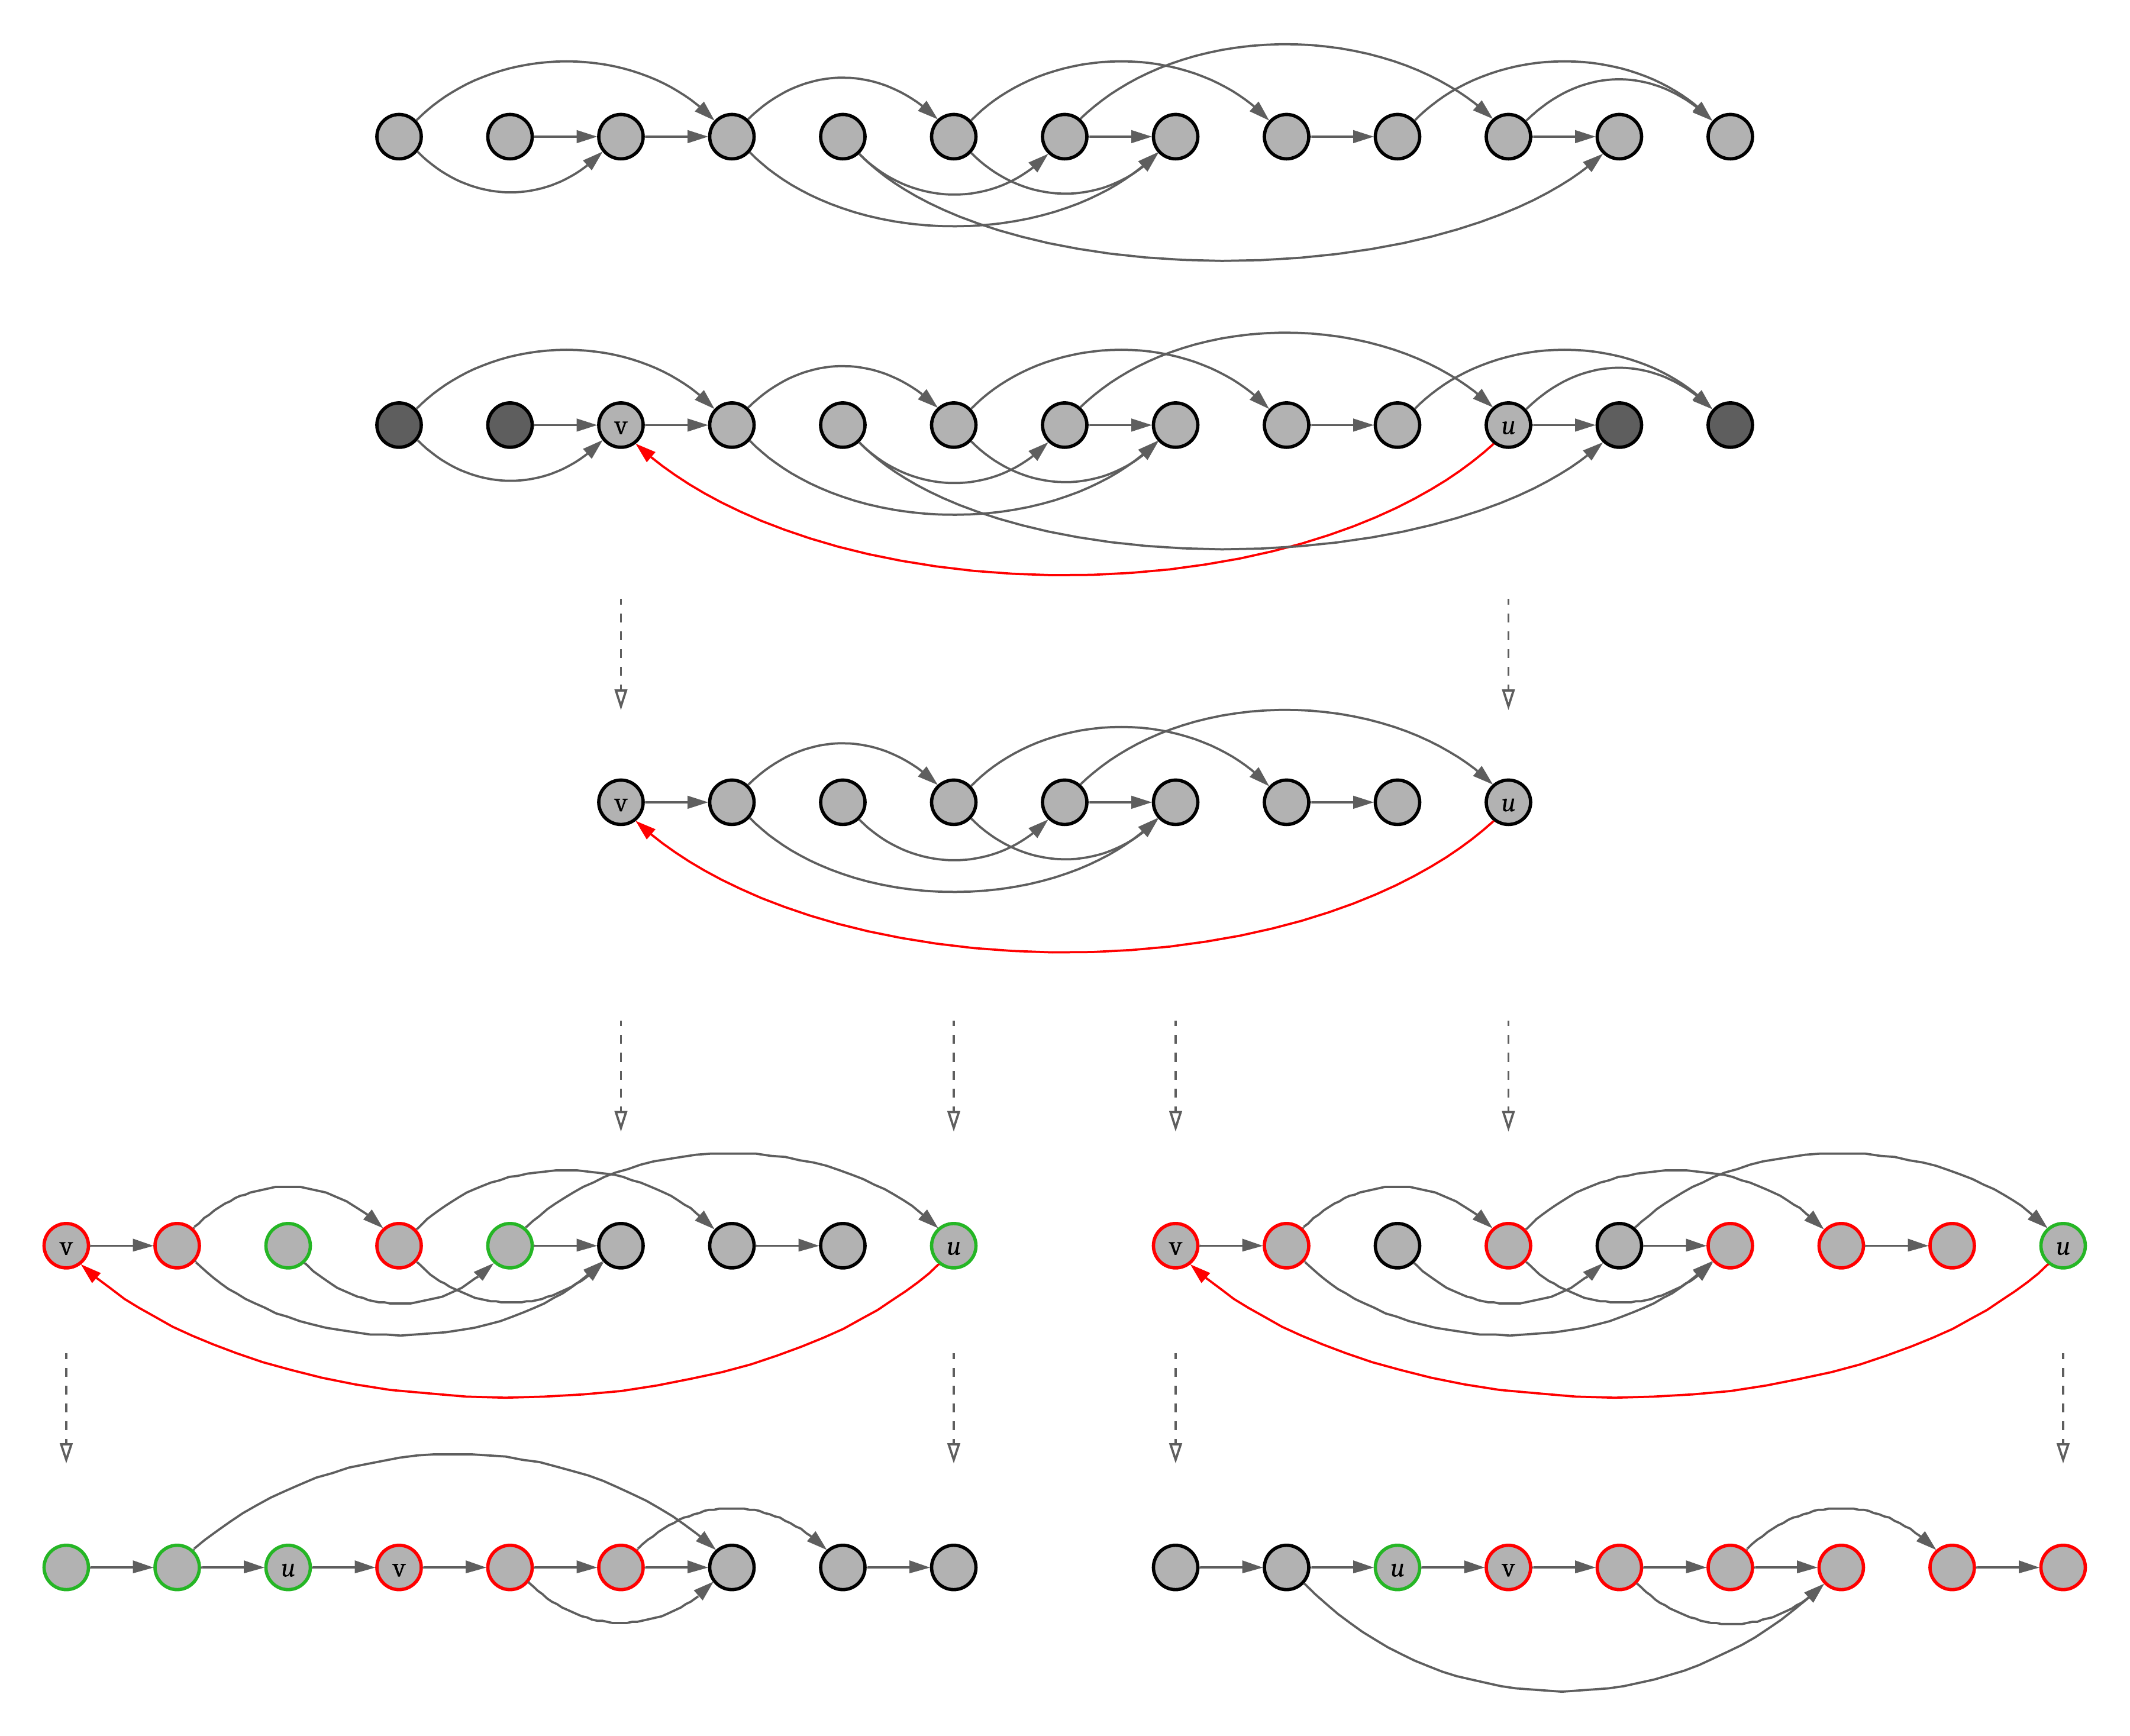
\includegraphics[width=16cm]{Images/Simple Algos.png}}
    \caption{A comparison of the simple search algorithms, one-way search $\pazocal A_1$ (right), and greedy two-way search $\pazocal A_2$ (left), restoring the topological ordering after the insertion of $(u,v)$ by rearranging nodes in the affected region.}
    \label{fig:simplesearch}
\end{figure}

\section{Open Problems}

There are many open problems related to incremental cycle detection and topological ordering, including some related to the notion of recourse which I have just introduced. Most of these are mainly concerned with obtaining amortized polylogarithmic update times in certain settings, the most important (and also the hardest) of which is the question of whether there exists an algorithm for incremental cycle detection with a worst case or expected runtime of $\tilde{\pazocal O}(m)$ on all inputs. While this problem is notoriously hard and far outside the scope of this project, there are other open problems that are more accessible. Before covering these, I will briefly discuss the \textit{random-order model}, and it's relevance to incremental cycle detection and topological ordering.

\subsection{Random Order Arrival vs. Adversarial Arrival}

In the \textit{random-order model} for dynamic algorithms, the input is chosen by an \textit{adversary} but is randomly permuted before being presented to the algorithm. This process of randomizing the order of the input can often weaken the power of the adversary.\footnote{Gupta el al. give a good survey of the random-order model and many examples in their paper \cite{GuptaS20}}

This model is very applicable in the context of incremental topological ordering; it's very natural to ask whether randomising the order of an insertion sequence before presenting it to some algorithm will provide us with improved algorithmic guarantees. I shall refer to this setting as \textit{random-order arrival} and the setting where the adversary has complete control over the insertion sequence as \textit{adversarial arrival}. My supervisor, Sayan Bhattacharya, has conjectured that there exists an incremental topological ordering algorithm that has low expected recourse per insertion for any graph under random-order arrival for any initial ordering. Where the expected recourse (given some inital ordering $\prec$) under random-order arrival is defined as follows.

\[ \mathbb{E}_{\pazocal E \in \mathcal{S}_{E}}[rec(\pazocal E, \prec)] = \sum_{j \geq 0} j \cdot \mathbb{P}[rec(\pazocal E, \prec)=j] = \frac{1}{m!} \sum_{\pazocal E \in \mathcal S_E}rec(\pazocal E, \prec) \]

More formally, we have the following conjecture.

\begin{conjecture}\label{mainconjecture}
Let $G=(V,E)$ be a DAG and $\prec \: \in \mathcal S_V$ any initial ordering of $G$, then there exists some incremental topological ordering algorithm such that it's recourse satisfies the following
\[ \mathbb E_{\pazocal E \in \mathcal S_E}[rec(\pazocal E, \prec)] = \tilde{\pazocal O}(m) \]
\end{conjecture}

In fact, he has conjectured that the algorithms $\pazocal A_1$ and $\pazocal A_2$ have low expected recourse \textit{per node} (not just per insertion) for any graph (and initial ordering) under random-order arrival. In contrast, note that insertion sequences leading to high recourse can easily be constructed for both of these algorithms under adversarial arrival (see \ref{locallowerbound}). More formally, we have the following conjectures.

\begin{conjecture}\label{A1conjecture}
Let $G=(V,E)$ be a DAG and $\prec \: \in \mathcal S_V$ any initial ordering of $G$, then the recourse of the simple one-way search algorithm, $\pazocal A_1$, satisfies the following
\[ \mathbb E_{\pazocal E \in \mathcal S_E}[rec(\pazocal E, \prec)] = \tilde{\pazocal O}(n) \]
\end{conjecture}

\begin{conjecture}\label{A2conjecture}
Let $G=(V,E)$ be a DAG and $\prec \: \in \mathcal S_V$ any initial ordering of $G$, then the recourse of the simple greedy two-way search algorithm, $\pazocal A_2$, satisfies the following
\[ \mathbb E_{\pazocal E \in \mathcal S_E}[rec(\pazocal E, \prec)] = \tilde{\pazocal O}(n) \]
\end{conjecture}

Since for both of these algorithms we can assume that the input graphs are weakly connected (it can be shown that the effect of either algorithm on some node $u \in V(G)$ only depends on the structure of $G[reach_G(u) \cup reach^{-1}_G(u)]$, so we only have to consider graphs which are weakly connected), we can assume without loss of generality that $m=\Omega(n)$. Hence, Conjecture \ref{A1conjecture} and \ref{A2conjecture} both individually imply Conjecture \ref{mainconjecture}.

\subsection{Experimental Results}\label{simplealgotests}

Before I started thinking about these problems, I implemented the simple algorithms, $\pazocal A_1$ and $\pazocal A_2$, and tested them on many randomly generated graphs.\footnote{All the code for these implementations can be found at github.com/martin-costa/incremental-cycle-detection} All the data I collected supports both of these conjectures. Figure \ref{fig:recoursetests1} shows some of the data. I have not included the details of how I generated the DAGs or the insertion sequences within this report since I want to focus on concrete results and not experimental data. However, I did try many different techniques and attained the same results each time. All of these tests can also be found in the repository referenced below.

\begin{figure}[htp]
    \centering
    \centerline{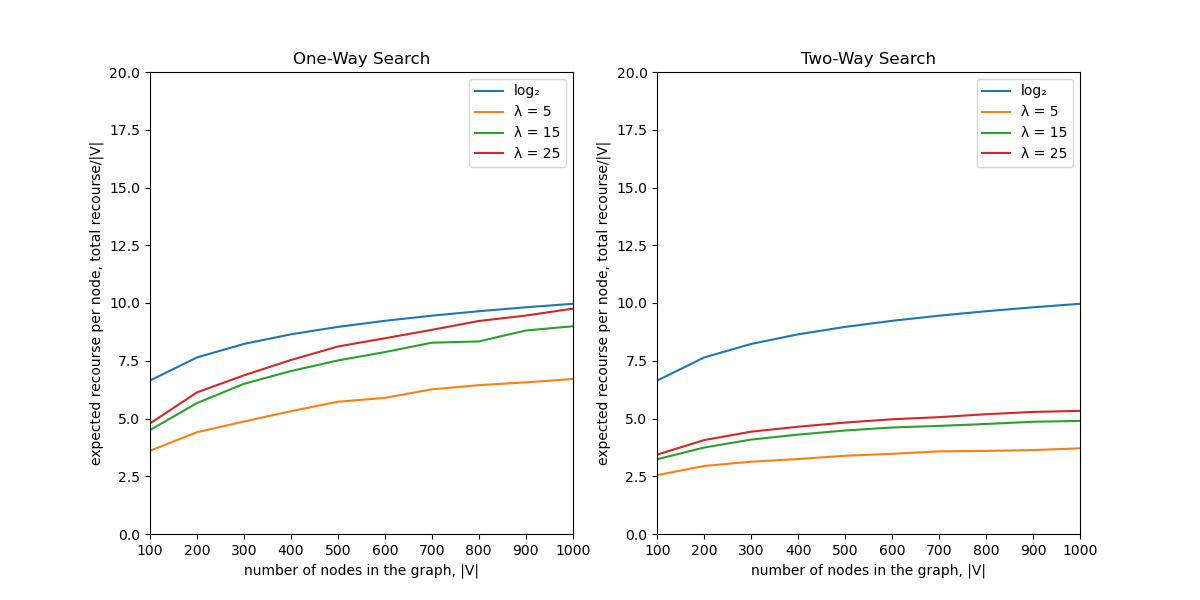
\includegraphics[width=18cm]{Images/simple algo tests.png}}
    \caption{The curve $\lambda = k$ shows the average recourse per node (with respect to $\pazocal A_1$ on the left and $\pazocal A_2$ on the right) over many randomly generated insertion sequences of length exactly $\lambda n$ on randomly generated DAGs with $n$ nodes.}
    \label{fig:recoursetests1}
\end{figure}

%%%%____%%%% CHAPTER 4 : DIVIDE AND CONQUER FRAMEWORK %%%%____%%%%
\chapter{Divide and Conquer Framework}\label{chapter4}

In this chapter I will be designing a divide and conquer framework for incremental cycle detection and topological ordering, which can be used to design divide and conquer algorithms to tackle the problem. I will use the ideas presented to construct a high level algorithm using the framework, and then see how it's recourse compares to $\pazocal A_1$ and $\pazocal A_2$ which we introduced in the last chapter. The reason this is relevant is that currently there are no known \textit{efficient implementations} of the simple search algorithms $\pazocal A_1$ or $\pazocal A_2$, i.e. implementations that give us a runtime close to their recourse, so this new framework could potentially yield algorithms with low expended recourse which can be implemented more efficiently.

\section{The Core Ideas}

I will start off by giving the definitions and propositions that are at the core of this framework. The main idea here is the notion I have defined as `semi-topological partitions', which will allow us to split the ordering into 3 sections in quite a natural way that breaks down the problem.

\subsection{Basic Definitions}

In order to create a divide and conquer framework for the problem, we need to be able to recursively break down the problem into smaller sub-problems, leading to the following natural definition.

\begin{definition}[Topological Partition]
Let $G=(V,E)$ be a DAG, then $(L,R)$ is a \textit{topological partition} of G if
\begin{enumerate}
\item L and R partition V, i.e. $L \cap R = \varnothing$ and $L \cup R = V$
\item adding any edge from R to L will create a cycle
\item there are no edges from $R$ to $L$
\end{enumerate}
\end{definition}

It turns out that this notion of topological partitions is too strict to be used directly; it is very easy to construct a DAG $G=(V,E)$ with $m=\Omega (n^{2})$ that has no non-trivial topological partitions. For example, suppose $u \in V$ and let $(L,R)$ be a partition of $V\setminus{\{u\}}$ with $\Theta(\vert L \vert)$ = $\Theta(\vert R \vert)$ = $\Theta(n)$ and $E = L \times R$. We can see that there can't be a topological partition of $G$ because $u$ is isolated in $G$, so adding any edge into the graph which is incident on $u$ would never create a cycle, even though $m=\Omega (n^{2})$.

However, even though a topological partition doesn't exist for G, we can see (at least intuitively) that G is \textit{almost} partitioned topologically by $(L,R)$, so I now give a relaxation of this definition that captures this formally.

% definition of an STP
\begin{definition}[Semi-Topological Partition]
Let $G=(V,E)$ be a DAG, then $(L,F,R)$ is a \textit{semi-topological partition} of $G$ with \textit{freedom} $\frac{1}{n} \vert F \vert$ if
\begin{enumerate}
\item $L$, $F$ and $R$ partition $V$
\item adding any edge from $R$ to $L$ will create a cycle
\item there are no edges from $F$ to $L$, from $R$ to $F$ or from $R$ to $L$, i.e. $\forall u \in F$, $u \notin reach_{G}^{-1}(L)$ and $u \notin reach_{G}(R)$, and $\forall u \in R$, $u \notin reach_{G}^{-1}(L)$ 
\end{enumerate}
\end{definition}

We can see that $(L,R)$ is a topological partition (TP) of $G$ if, and only if, $(L,\varnothing,R)$ is a semi-topological partition (STP) of $G$. More importantly, we can see that this new notion of STPs does not have the same limitations as the notion of TPs. In fact, any non-empty DAG has a non-trivial STP.

\subsection{Properties of STPs}

We will now make some observations about the properties of STPs. In the next section we will discuss how we can use these properties to construct a divide and conquer algorithm using the idea of STPs as a foundation.

\begin{proposition}
Let $G=(V,E)$ be a DAG, given disjoint $L,R \subseteq V$, the following are equivalent
\begin{enumerate}
\item adding any edge from $R$ to $L$ will create a cycle
\item $\forall u \in L$, $v \in R$ we have $v \in reach_{G}(u)$
\item $L \subseteq \bigcap_{u \in R} reach_{G}^{-1}(u)$
\item $R \subseteq \bigcap_{u \in L} reach_{G}(u)$
\end{enumerate}
\end{proposition}

\begin{proof}
$\textbf{1.} \Leftrightarrow \textbf{2.}$ If adding any edge from $R$ to $L$ creates a cycle, then from any node in $L$ we can reach any node in $R$. If from any node in $L$ we can reach any node in $R$, then adding any edge $(v,u)$ from $R$ to $L$ will create a cycle, since we can append this edge to the end of a path from $u$ to $v$.

$\textbf{2.} \Leftrightarrow \textbf{3.}$ and $\textbf{2.} \Leftrightarrow \textbf{4.}$ are obvious.
\end{proof}

\begin{proposition}
Let $G=(V,E)$ be a DAG. Suppose $(L,F,R)$ is an STP of $G$, then
\begin{enumerate}
\item $\forall u \in L$, $reach_{G}^{-1}(u) \subseteq L$
\item $\forall u \in R$, $reach_{G}(u) \subseteq R$
\end{enumerate}
\end{proposition}

\begin{proof}
\textbf{1.} Suppose $u \in L$ and $v \in reach_{G}^{-1}(u)$, if $v \notin L$ then there is a path from $v \in F \cup R$ to $u$, hence there exists an edge from $F$ to $L$ or from $R$ to $L$ giving a contradiction, hence $reach_{G}^{-1}(u) \subseteq L$. \textbf{2.} Same argument as \textbf{1.}
\end{proof}

This next Lemma will be useful for finding STPs, it will give us a very simple way to construct an STP by looking at any edge in the graph.

\begin{lemma}[Simple STP Construction]
Let $G=(V,E)$ be a DAG, let $u \in V$ and $v \in reach_{G}(u)$, then
\begin{enumerate}
\item if $u \neq v$ then $(reach_{G}^{-1}(u),F,reach_{G}(v))$ is an STP of $G$
\item if $u = v$ then $(reach_{G}^{-1}(u),F,reach_{G}(u) \setminus{\{u\}})$ and $(reach_{G}^{-1}(u) \setminus{\{u\}},F,reach_{G}(u))$ are STPs of $G$
\end{enumerate}
with $F=V \setminus (reach_{G}^{-1}(u) \cup reach_{G}(v))$
\end{lemma}

\begin{proof}
\textbf{1.} Let $L=reach_{G}^{-1}(u)$ and $R=reach_{G}(v)$. If $L \cap R \neq \varnothing$ then $u \in reach_{G}(v)$ so $G$ contains a cycle, contradicting the fact that $G$ is a DAG. So $L$, $F$ and $R$ partition $V$. If we add any edge $(v^{*},u^{*})$ from $R$ to $L$, since we can form paths from $u^{*} \rightsquigarrow u$, $u \rightsquigarrow v$ and $v \rightsquigarrow v^{*}$, we can append these paths together along with $(v^{*},u^{*})$ to obtain a cycle. Let $w \in F$ and suppose $w \in reach_{G}^{-1}(L) = reach_{G}^{-1}(u)$, then by the definition of $L$, $w \in L$, giving a contradiction, so there are no edges from $F$ to $L$. Similarly, there are no edges from $R$ to $F$ or from $R$ to $L$ since $R$ and $L$ are disjoint. It follows that $(reach_{G}^{-1}(u),F,reach_{G}(v))$ is an STP of $G$.
\textbf{2.} Same argument as 1.
\end{proof}

We refer to an STP that has one of the forms just discussed as a \textit{simple} STP. Given any DAG with at least one edge, we can now construct an STP of the graph by simply taking any edge $e$ and applying the Lemma above to it's endpoints, we call this the \textit{simple STP constructed by $e$}. This Lemma will be crucial in the construction of the algorithm which I will give later.

This next Lemma formalises the main reason that the notion of STPs is useful for this problem. It follows directly from the definition of an STP so it's quite trivial, but it's important so we say it explicitly anyway.

\begin{lemma}
Let $G=(V,E)$ be a DAG. Suppose $(L,F,R)$ is an STP of $G$ and that $\prec_{L}$, $\prec_{F}$ and $\prec_{R}$ are topological orderings of $G[L]$, $G[F]$ and $G[R]$ respectively. The ordering $\prec_{G}$ that we get from combining these topological orderings and setting $L \prec_{G} F \prec_{G} R$ is a topological ordering of $G$. Formally, given $u, v \in G$, if for some $S \in \{ L,F,R\}$ $u,v \in S$ then $u \prec_{G} v$ if $u \prec_{S} v$, else $u \prec_{G} v$ if $u \in L$ or if $u \in F$ and $v \in R$. 
\end{lemma}

\begin{proof}
Follows directly from the definition of a topological ordering combined with the definition of an STP.
\end{proof}

% CHAPTER 2
\section{Constructing the Framework}

In this section I will present a structure that can be updated incrementally alongside the graph as edge insertions are made. This structure will be constructed by recursively computing embedded STPs, and will allow us to maintain a topological ordering of the graph by maintaining this system of embedded STPs (and taking advantage of their properties) instead of maintaining a topological ordering directly. I will then show how this structure can be used to design an algorithm for incremental cycle detection and topological ordering. 

To make things easier to read, for the rest of this chapter fix a DAG $G=(V,E)$ and an insertion sequence $\pazocal E \in \mathcal S_E$ of $G$. As usual, we start with the graph $G_{0}=(V,\varnothing)$ and add edges from $\pazocal E$ one at a time. Let $G_{t}$ denote the graph after $t$ edge insertions from $\pazocal E$, i.e. the graph $(V,\{\pazocal E_{1},...,\pazocal E_{t}\})$.

\subsection{The Meta Tree}

As we incrementally perform edge insertions, we also maintain a rooted meta-tree $\pazocal T$ which captures information about STPs that we will compute along the way, helping us to classify the edge insertions that are being performed into various types and to (indirectly) maintain a topological ordering of the graph.

Let $\pazocal T_t$ denote the state of the meta-tree after the first $t$ insertions. All of the internal meta-nodes $x$ of $\pazocal T_t$ have exactly 3 children, the left, middle and right, denoted by $x_L$, $x_F$ and $x_R$ respectively. The meta-leaves of $\pazocal T_t$ all have ordered subsets of $V(G)$ \textit{attached} to them, given a meta-leaf $x$ of $\pazocal T_t$, we denote this set by $set_t(x)$ and the ordering of this set by $\prec_t^x$. We also recursively define $set_t$ for internal meta-nodes $x$ by setting $set_t(x) = set_t(x_L) \cup set_t(x_F) \cup set_t(x_R)$ with the ordering of $set_t(x)$ induced from the orderings of the $set_t$ of its children and setting $set_t(x_{L}) \prec_t^x set_t(x_{F}) \prec_t^x set_t(x_{R})$.

We want to construct and update the meta-tree, $\pazocal T$, in such that it always satisfies certain properties, making it useful to us. These invariants are as follows.

\begin{invariant}[The Meta Tree Properties]
The meta-tree $\pazocal T$ maintains the following properties as edges are inserted, $\forall \: t \in \{0,...,m\}$:

\begin{enumerate}
\item The subsets of $V$ attached to the meta-leaves of $\pazocal T_t$ form a partition of $V$
\item Given any meta-node $x$ of $\pazocal T_t$, the ordering $\prec_t^x$ is a topological ordering on $G_t[set_t(x)]$
\item Given any internal meta-node $x$ of $\pazocal T_t$, $(set_t(x_L), set_t(x_F), set_t(x_R))$ is an STP of $G_t[set_t(x)]$
\item Let $x$ be a meta-node of $\pazocal T_t$, if the (unique) path from $x$ to the root doesn't contain any meta-nodes that are middle children, then for any $s\geq t$, $set_t(x) \subseteq set_s(x)$
\end{enumerate}
\end{invariant}

The meta-tree $\pazocal T_0$ is a single meta-node $r$ with $set_t(r)=V(G)$ and any random ordering of the nodes $\prec_t^r$. We want to find an algorithm that allows us to efficiently compute $\pazocal T_t$ from $\pazocal T_{t-1}$ and $G_t$ such that $\pazocal T_t$ satisfies all the meta properties, giving us $\prec_t^r$ which by properties 2 and 3 of the meta-tree defines a topological ordering on $G_t$.

% edge insertions
\subsection{Handling Edge Insertions}

I will now describe, at a high level, how we can update the meta-tree after an insertion has occurred such its properties are all preserved. I will show how edges can be classified into different types and what has to be done to handle each type of edge insertion. 

Let $\prec_t^{meta}$ be an ordering of the meta-leaves of the meta-tree created by traversing $\pazocal T_t$ in pre-order, so for any two meta-leaves $x,y \in V(\pazocal T_t)$, $x \prec_t^{meta} y$ if $x$ is explored before $y$ in the pre-order traversal of $\pazocal T_t$. Notice that if we combine $\prec_t^{meta}$ with the orderings $\prec_t^x$ for the sets $set_t(x)$ at each meta-leaf $x$, we get $\prec_t^r$. For some node $u \in V(G)$, let $node_t(u)$ denote the unique meta-leaf $x$ in $\pazocal T_t$ that has $u \in set_t(x)$.

Let $\pazocal E_t=(u_t,v_t)$ be the edge inserted at step $t$ into $G_{t-1}$ to obtain $G_t$. Let $p_t = (x_1,...,x_k)$ be the unique path from $x_1 = node_{t-1}(u_t)$ to $x_k = node_{t-1}(v_t)$ in $\pazocal T_{t-1}$. Let $x_j\in p_t$ denote the least common ancestor of $x_1$ and $x_k$ in $\pazocal T_{t-1}$. We now consider the 3 following cases that may occur when an edge is inserted.

\begin{enumerate}
\item $node_{t-1}(u_t) \prec_{t-1}^{meta} node_{t-1}(v_{t})$
\item $node_{t-1}(u_t) = node_{t-1}(v_t)$
\item $node_{t-1}(v_t) \prec_{t-1}^{meta} node_{t-1}(u_t)$ 
\end{enumerate}

Here is an outline of what has to be done to restore or maintain the properties of the meta-tree in these 3 cases.

% forward edge
\subsubsection{Case $node_{t-1}(u_t) \prec_{t-1}^{meta} node_{t-1}(v_{t})$:}

If this is the case, then we don't need to do anything since $x_{1} \prec_{t-1}^{meta} x_{k}$ so $u_t \prec_{t-1}^r v_t$. So we can just let $\pazocal T_t= \pazocal T_{t-1}$.

% same set edge
\subsubsection{Case $node_{t-1}(u_t) = node_{t-1}(v_t)$:}

If this is the case, then we can apply the simple STP construction Lemma to $(u_t,v_t)$ and break down the set $S=set_{t-1}(x)$ with $x=node_{t-1}(u_t)$ into an STP $(L,F,R)$, with $L=reach_t^{-1}(u_t) \cap S$, $R=reach_t(v_t) \cap S$ and $F=S \setminus (L \cup R)$. To compute $\pazocal T_t$, take $\pazocal T_{t-1}$ and add 3 children, $x_{L}$, $x_{F}$ and $x_{R}$ to $x$ with $set_t(x_{L}) = L$, $set_t(x_{F}) = F$ and $set_t(x_{R}) = R$, with the orderings of these sets induced by restricting $\prec_{t-1}^{x}$ to $L$, $F$ and $R$ respectively.

% backwards edge
\subsubsection{Case $node_{t-1}(v_t) \prec_{t-1}^{meta} node_{t-1}(u_t)$:}

This case is by far the most complex, since we need to be able to remove and add nodes to STPs in such a way that preserve the invariant properties of the meta-tree. Immediately we can observe that since $node_{t-1}(u_t) \npreceq^{meta}_{t-1} node_{t-1}(v_t)$ we have $u_t \nprec^{r}_{t-1} v_t$, hence $\pazocal T_t \neq \pazocal T_{t-1}$.

In the next section we will show how to recursively add sets of topologically ordered nodes into the sets attached to sub-trees of the meta-tree while maintaining the properties of the meta-tree. For now just assume it's possible. Consider the state of $\pazocal T_{t-1}$ around the meta-node $x_j$ defined above. Since we have $node_{t-1}(v_t) \prec_{t-1}^{meta} node_{t-1}(u_t)$, there are 3 possibilities for where $x_{j-1}$ and $x_{j+1}$ are located. By definition of $x_j$ we have $x_{j-1}, x_{j+1} \in \{ x_{j}_{L}, x_{j}_{F}, x_{j}_{R} \}$. Now consider the 3 cases.

\begin{enumerate}
    \item $x_{j-1}=x_{j}_{R}$ and $x_{j+1}=x_{j}_{L}$: we can immediately deduce that a cycle is present in $G_t$ since an edge has been added from the \textit{right} nodes to the \textit{left} nodes of the STP associated with the meta-node $x_{j}$
    
    \item $x_{j-1}=x_{j}_{R}$ and $x_{j+1}=x_{j}_{F}$: remove $reach_t(v_t) \cap set_{t-1}(x_{j}_{F})$ from $set_{t-1}(x_{j}_{F})$ and add it to $set_{t-1}(x_{j}_{R})$.
    
    \item $x_{j-1}=x_{j}_{F}$ and $x_{j+1}=x_{j}_{L}$: remove $reach_t^{-1}(u_t) \cap set_{t-1}(x_{j}_{F})$ from $set_{t-1}(x_{j}_{F})$ and add it to $set_{t-1}(x_{j}_{L})$.
\end{enumerate}

So we can fully restore the properties of the meta-tree (and hence the topological ordering of the graph that is induced by the meta-tree) with a single call to this (currently undefined) algorithm that moves nodes between the STPs in the meta-tree.

\section{Computing the Meta Trees}

We will now give a high level algorithm that will allow us to recursively move topologically ordered sets of nodes between the sets attached to meta-nodes in the meta-tree where necessary, while also maintaining the properties of the meta-tree. Combining this with the algorithm given in the last section that required the ability to perform this operation, we will have constructed a high level divide and conquer algorithm for incremental cycle detection and topological ordering.

Similar to the simple algorithms $\pazocal A_1$ and $\pazocal A_2$, I will not be giving any concrete implementation of this algorithm using data structures and so on. The description that I have given of this algorithm is all that is required to study it's combinatorial properties, such as the recourse of this algorithm in different settings, which is currently my main interest. 

\subsection{Modifying the STPs of the Meta Tree}

As we saw in the last section, in some cases, we need to be able to move nodes between the sets attached to the meta-leaves of the meta-tree. Here we give a high level algorithm that will allow us to do this. In particular, we want an algorithm that given a meta-node $x$ in $\pazocal T_{t-1}$, allows us to move topologically ordered subsets $A \subseteq \bigcup_{y \prec^{meta}_{t-1} x} set_{t-1}(y)$ and $B \subseteq \bigcup_{x \prec^{meta}_{t-1} y} set_{t-1}(y)$ with orderings $\prec_{A}$ and $\prec_{B}$ respectively, into $S=set_{t-1}(x)$, with the sets satisfying the following properties\footnote{Here we extend the ordering $\prec^{meta}_t$ to pairs of unrelated meta-nodes in $\pazocal T_t$ in the obvious way, where $x \prec^{meta}_t y$ if $x$ is explored before $y$ in the pre-order traversal of $\pazocal T_t$}

\begin{enumerate}
\item $A$, $B$ and $S$ are pairwise disjoint
\item the ordering $\prec^{*}$ we get from combining $\prec_{A}$, $\prec_{B}$ and $\prec_{t-1}^x$ and setting $A \prec^{*} S \prec^{*} B$ disagrees with at most one edge in $G_t$ between the sets
\end{enumerate}

We now give an outline for an algorithm ADD$(\pazocal T,G_t,x,A,B)$ in algorithm \ref{ADD} which takes the current meta-tree $\pazocal T$ (which may not satisfy the meta-tree properties after the insertion of $\pazocal E_t$), the graph $G_t$, a meta-node $x$ in $\pazocal T$, two sets of nodes $A$ and $B$ satisfying the properties above, and moves the nodes in $A$ and $B$ into the meta-leaves in the sub-tree of $x$. We will later see that a single call of this algorithm can restore all the properties of the meta-tree after an insertion, more specifically, it can compute $\pazocal T_t$ from $\pazocal T_{t-1}$ and $G_t$ after a type 3 edge insertion.

Note that up to know we have been considering the meta-tree at specific states, i.e. we have only cared about $\pazocal T_0, \pazocal T_1,..., \pazocal T_m$, and considered (at a high level) how we have to modify the meta-tree $\pazocal T$ starting from $\pazocal T_{t-1}$ to get to a state where it satisfies the meta-tree properties for the updated graph $G_t$. We will now have to consider the state of the meta-tree as me modify it to transition between these \textit{nice} states, so the notation will be slightly different. We just generalise the notation from these specific states of the meta-tree to the meta-tree at any state in the obvious way by replacing $\prec_t^x$ with $\prec_{\pazocal T}^x$, $set_t(x)$ with $set_{\pazocal T}(x)$, and so on.\newline

% \begin{enumerate}
%     \item \textbf{Base case.} If $x$ is not an internal meta-node of $\pazocal T$ (i.e. $x$ is a meta-leaf), then let $set_{\pazocal T}(x)=A\cup set_{\pazocal T}(x)\cup B$, and let $\prec_{\pazocal T}^{x}$ be the ordering we get from combining the other orderings as done above. If there is an edge that disagrees with this ordering, i.e. this is not a topological ordering on $set_{\pazocal T}(x)$, then treat this like a type 2 edge insertion. 
%     \item \textbf{Recursive call.} First we create 6 ordered sets that we will use to partition $A$ and $B$. $L_{A}$, $F_{A}$ and $R_{A}$ for $A$ and $L_{B}$, $F_{B}$ and $R_{B}$ for $B$ initially all $\varnothing$. Let $L$, $F$ and $R$ denote $set_{\pazocal T}(x_{L})$, $set_{\pazocal T}(x_{F})$ and $set_{\pazocal T}(x_{R})$ respectively.
%     \item \begin{enumerate}[i.] 
%         \item Find $reach_{t}^{-1}(L) \cap A$, remove it from $A$, and place it in $L_{A}$
%         \item Find $reach_{t}^{-1}(L) \cap B$, remove it from $B$, and place it in $L_{B}$
%         \item Find $reach_{t}(R) \cap A$, remove it from $A$, and place it in $R_{A}$
%         \item Find $reach_{t}(R) \cap B$, remove it from $B$, and place it in $R_{B}$
%         \end{enumerate}
%     \item \begin{enumerate}[i.] 
%         \item Find $reach_{t}^{-1}(L_{A} \cup L_{B}) \cap F$, remove it from $F$, and place it in $L_{B}$
%         \item Find $reach_{t}(R_{A} \cup R_{B}) \cap F$, remove it from $F$, and place it in $R_{A}$
%         \end{enumerate}
%     \item Let $F_{A}=A \setminus (L_{A} \cup R_{A})$ and $F_{B}=B \setminus (L_{B} \cup R_{B})$
%     \item \begin{enumerate}[i.] 
%         \item recursive call to ADD$(\pazocal T, G_t, x_{L},L_{A},L_{B})$
%         \item recursive call to ADD$(\pazocal T,G_t, x_{F},F_{A},F_{B})$
%         \item recursive call to ADD$(\pazocal T,G_t, x_{R},R_{A},R_{B})$
%         \end{enumerate}
% \end{enumerate}

\begin{algorithm}[H]\label{ADD}
    \SetAlgoLined
    $\triangleright$ \textbf{STEP 1: Base case}
    
    If $x$ is not an internal meta-node of $\pazocal T$ (i.e. $x$ is a meta-leaf), then let $set_{\pazocal T}(x)=A\cup set_{\pazocal T}(x)\cup B$, and let $\prec_{\pazocal T}^{x}$ be the ordering we get from combining the other orderings as done above. If there is an edge that disagrees with this ordering, i.e. this is not a topological ordering on $set_{\pazocal T}(x)$, then treat this like a type 2 edge insertion.
    
    $\triangleright$ \textbf{STEP 2: Recursive call}
    
    First we create 6 ordered sets that we will use to partition $A$ and $B$. $L_{A}$, $F_{A}$ and $R_{A}$ for $A$ and $L_{B}$, $F_{B}$ and $R_{B}$ for $B$ initially all $\varnothing$. Let $L$, $F$ and $R$ denote $set_{\pazocal T}(x_{L})$, $set_{\pazocal T}(x_{F})$ and $set_{\pazocal T}(x_{R})$ respectively.
    \caption{ADD$(\pazocal T,G_t,x,A,B)$}
    
    $\triangleright$ \textbf{STEP 3}
    
    Find $reach_{t}^{-1}(L) \cap A$, remove it from $A$, and place it in $L_{A}$\;
    Find $reach_{t}^{-1}(L) \cap B$, remove it from $B$, and place it in $L_{B}$\;
    Find $reach_{t}(R) \cap A$, remove it from $A$, and place it in $R_{A}$\;
    Find $reach_{t}(R) \cap B$, remove it from $B$, and place it in $R_{B}$\;
    
    $\triangleright$ \textbf{STEP 4}
    
    Find $reach_{t}^{-1}(L_{A} \cup L_{B}) \cap F$, remove it from $F$, and place it in $L_{B}$\;
    Find $reach_{t}(R_{A} \cup R_{B}) \cap F$, remove it from $F$, and place it in $R_{A}$\;
    
    $\triangleright$ \textbf{STEP 5}
    
    Let $F_{A}=A \setminus (L_{A} \cup R_{A})$ and $F_{B}=B \setminus (L_{B} \cup R_{B})$\;
    
    $\triangleright$ \textbf{STEP 6}
    
    recursive call to ADD$(\pazocal T, G_t, x_{L},L_{A},L_{B})$\;
    recursive call to ADD$(\pazocal T,G_t, x_{F},F_{A},F_{B})$\;
    recursive call to ADD$(\pazocal T,G_t, x_{R},R_{A},R_{B})$\;
\end{algorithm}

\subsection{Correctness}

I will now be giving a brief informal justification of the correctness of the high level algorithm we have constructed, which we shall refer to as $\pazocal A_D$. I have decided not to include the full formal argument since I do not believe it is insightful and the proofs are all very similar and fairly trivial. I have, however, included formal proofs of the most important propositions.

As we saw, all internal meta-nodes $x$ of $\pazocal T_t$ have associated STPs on $G_t[set_t(x)]$. We want our algorithm to reduce the \textit{freedom} of these STPs when possible, and the process which we use to do this requires the following proposition.

\begin{proposition}
Let $G=(V,E)$ be a DAG. Suppose $(L,F,R)$ is an STP of $G$ with $u \in V$, $D=reach_{G}(u)$, $A=reach_{G}^{-1}(u)$ then $(L\setminus D,F\setminus D,R\setminus D)$ is an STP of $G[V\setminus D]$ and $(L\setminus A,F\setminus A,R\setminus A)$ is an STP of $G[V\setminus A]$
\end{proposition}

\begin{proof}
Let $P=(L\setminus D,F\setminus D,R\setminus D)$. We need to check the 3 conditions of an STP. \textbf{1.} Since $L$, $F$ and $R$ partition $V$, we get that $L\setminus D$, $F\setminus D$, and $R\setminus D$ partition $V\setminus D$. \textbf{3.} There can't be any edges from $F\setminus D$ to $L\setminus D$, from $R\setminus D$ to $F\setminus D$, or from $R\setminus D$ to $L\setminus D$, or else this would contradict the fact that $(L,F,R)$ is an STP. \textbf{2.} Denote $G[V\setminus D]$ by $H$. Using the properties of an STP, we just need to show that $\forall v \in L \setminus D$, $w \in R \setminus D$ we have $w \in reach_{H}(v)$. Suppose this is not the case, then some $w \in R \setminus D$ can't be reached from some $v \in L \setminus D$ in $H$. Since $w \in reach_{G}(v)$, there exists some path $p$ from $v$ to $w$ in $G$. Since $p \nsubseteq V \setminus D$ we get that $p \cap D \neq \varnothing$, so let $u^{*} \in p \cap D$. Since $reach_{G}(u^{*}) \subseteq D$, $p \cap D$ is a path from $u^{*}$ to $w$ contained in $D$, hence $w \in D$, contradicting the fact that $w \in R \setminus D$. Hence, adding any edge from $R \setminus D$ to $L \setminus D$ creates a cycle. It follows that $P$ is an STP of H. An analogous argument gives the same for the STP $(L\setminus A,F\setminus A,R\setminus A)$ of $G[V\setminus A]$.
\end{proof}

\section{Results}

\subsection{Implications of the Framework}

Since this framework can be used to construct non-local algorithms that perform well experimentally on random graphs, it is possible that it could be used to construct non-local algorithms that perform well under adversarial arrival. $\pazocal A_D$ is a very simple example of an algorithm that can be created using this framework, and it does not perform well under adversarial arrival (it is easy to construct an insertion sequence that leads to $\Omega(n^2)$ recourse by creating $\Omenga(n)$ embedded STPs with very high freedom, and then recursively moving all the nodes in the deepest STP into the next deepest with one insertion).

\subsection{Experimental Results}

While I was unable to prove that this algorithm has an average expected recourse of $\pazocal O(\polylog n)$ per insertion, I did implement the algorithm $\pazocal A_D$ and test it in the same way as the simple algorithms in section \ref{simplealgotests}.\footnote{All the code for these implementations can be found at github.com/martin-costa/incremental-cycle-detection} Figure \ref{fig:recoursetests2} show some of the data I collected. All the data collected supports that $\pazocal A_D$ may give low expected recourse under random order arrival for any DAG. This implies that $\pazocal A_D$ is a candidate algorithm that could be used to prove Conjecture \ref{mainconjecture}.

\begin{figure}[htp]
    \centering
    \centerline{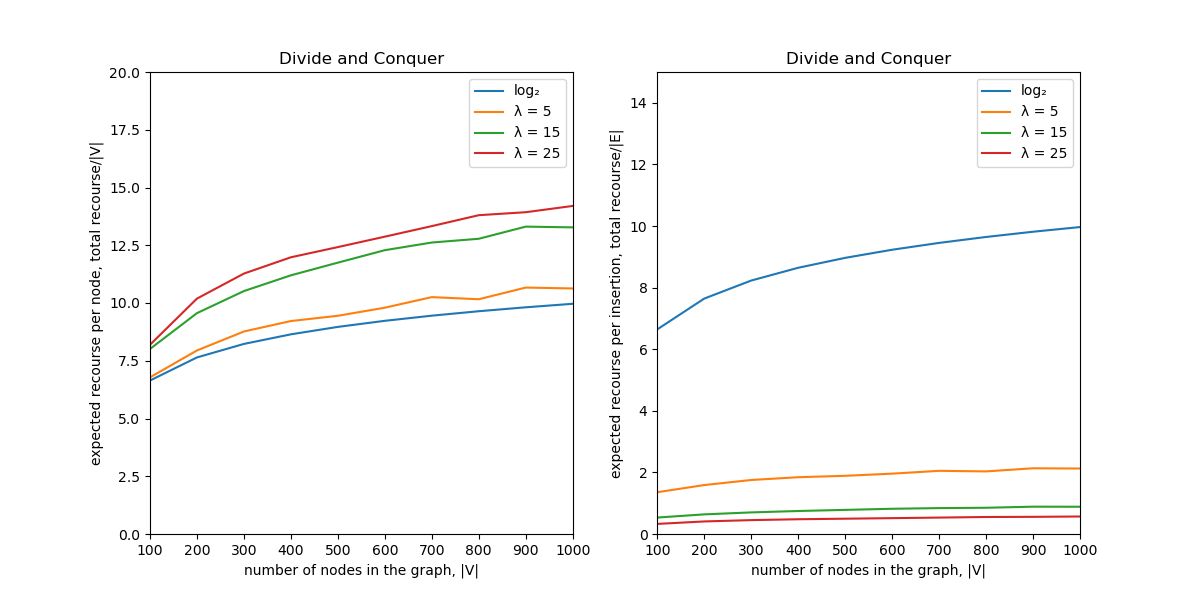
\includegraphics[width=18cm]{Images/DnCtests.png}}
    \caption{The curve $\lambda = k$ shows the average recourse of the divide and conquer algorithm per node (left) and per insertion (right) over many randomly generated insertion sequences of length exactly $\lambda n$ on randomly generated DAGs with $n$ nodes.}
    \label{fig:recoursetests2}
\end{figure}

%%%%____%%%% CHAPTER 5 : Random Order Arrival %%%%____%%%%
\chapter{Breaking Lower Bounds with Random-Order Arrival}\label{chapter5}

In this chapter I will be expanding on the claims I made at the end of chapter 4. In particular, I shall be covering the lower bound on recourse for \textit{local algorithms} that I briefly mentioned earlier as well as focusing on random order arrival. I will start off by giving an upper bound on the worst case recourse for $\pazocal A_2$, and then deducing this bound is tight since $\pazocal A_2$ is a local algorithm. I will then show that under random-order arrival, the lower bound on recourse for local algorithms given in \cite{HaeuplerKMST12} does not hold for $\pazocal A_2$. To make things simpler, I will only be focusing on the most important case where the input graphs are sparse, since the problem is well understood for dense graphs.

% SECTION 1
\section{Upper Bound on the Recourse of $\pazocal A_2$ }

We will now give an upper bound on the recourse of the simple greedy 2-way search algorithm, $\pazocal A_2$. While proofs of this bound already exist using similar arguments that rely on the same ideas, my proof uses the following potential function. For any graph $H$, define $\Psi(H) \triangleq \sum_{u \in V(H)}\vert reach_{H}(u) \vert \leq n^{2}$.

\begin{proposition}
Given any DAG $G=(V,E)$, the recourse of the simple greedy 2-way search algorithm, $\pazocal A_2$, satisfies the following.

\[ \max_{\pazocal E \in \mathcal S_E, \prec \in \mathcal S_V} rec(\pazocal E, \prec) =  \pazocal O (n \sqrt m) \]
\end{proposition}

\begin{proof}

Fix some DAG $G=(V,E)$ and any $\pazocal E \in \mathcal S_E$, $\prec \: \in \mathcal S_V$. Suppose that during the run of $\pazocal A_2$ on input $\pazocal E$ staring with initial ordering $\prec$, the edge $\pazocal E_t = (u,v)$ is inserted causing the total recourse to increase by $\lambda = rec(\pazocal E, \prec)_t$. Let $D$ denote the descendants of $v$ discovered by the forward search done by the algorithm during the insertion, and $A$ denote the ancestors of $u$ discovered by the backwards search done by the algorithm during the insertion. Let $a = \vert A \vert$ and $d = \vert D \vert$. Before the insertion, at most one node in $D$ could reach at most one node in $A$, but after the insertion, all of the nodes in $D$ can reach all of the nodes in $A$. So the descendants of at least $a-1$ nodes increase by at least $d - 1$. Combined with the fact that $\vert a - d \vert \leq 1$ and $\lambda \leq a + d$ we get that
\[ \Big (\frac{\lambda - 1}{2} - 1 \Big )^2 \leq (a-1)(d-1) \leq \Psi(G^{\pazocal E}_t) - \Psi(G^{\pazocal E}_{t-1}) \]

Summing over $t \in [m]$ on both sides of the inequality gives

\[ \sum_{t=1}^m \Big (\frac{rec(\pazocal E, \prec)_t - 1}{2} - 1 \Big )^2 \leq \Psi(G^{\pazocal E}_m) - \Psi(G^{\pazocal E}_{0}) \]

Using a simple norm bound and noticing that $\Psi(G_{0}^{\pazocal E})=0$ we get
\[ \sum_{t=1}^m \Big (\frac{rec(\pazocal E, \prec)_t - 1}{2} - 1 \Big ) \leq \Bigg (m \sum_{t=1}^m \Big (\frac{rec(\pazocal E, \prec)_t - 1}{2} - 1 \Big )^2 \Bigg )^{\frac{1}{2}} \leq \sqrt{m\Psi(G)} \leq n \sqrt m \]

Moving some terms to the right we get $rec(\pazocal E, \prec) \leq 3m + 2n \sqrt m = \pazocal O (n \sqrt m)$.
\end{proof}

% SECTION 2
\section{Lower Bound on the Recourse of Local Algorithms}

In the work of \cite{HaeuplerKMST12}, they construct a collection of both sparse and dense DAGs $\{ H_{k,p} : p,k \in \mathbb N, p \leq k \}$ with $n = \Theta(pk)$, $m=\Theta (k(k+p))$, with corresponding insertion sequences and initial orderings such that the recourse of \textit{any} local algorithm (recall definition \ref{localalgo}) is $\Omega(n\sqrt{m})$ on these inputs. I will now define these instances and show that they lead to high recourse. To make things simpler, since the problem is already well understood for dense graphs, I will only be considering the more important cases where the graphs are sparse, so we will only care about $\{H_{k,k}\}$ where $p=k$ (note that the sparse graphs $\{H_{1,p}\}$ where $k=1$ are just paths of length $\Theta(p)$ and not very interesting).\footnote{I have introduced the graphs in a slightly different way to \cite{HaeuplerKMST12} to make them easier to work with, but they are fundamentally the same}

\subsection{High Recourse Instances}

Fix some $k \in \mathbb{N}$, abbreviate $H_{k,k}$ to $H_k$ and let $H_k=(V,E)$. We can construct the graph $H_k$ with corresponding insertion sequence, $\pazocal E \in \mathcal S_E$, and initial ordering, $\prec \: \in \mathcal S_V$, such that $rec(\pazocal E, \prec) = \Omega(n\sqrt n)$ as follows.

\subsubsection{Constructing the Graph}

For all $i \in [k]$ let $S_{i} = \{ x_{i}, z_{i}^{2}, ..., z_{i}^{k-1}, y_{i} \}$ be sets of nodes of size $k$ and set $V = \bigcup_{i=1}^{k}S_{i}$. Starting with $E= \varnothing$, for all $i \in [k]$ add the edges $(x_{i}, z_{i}^{2}), (z_{i}^{2}, z_{i}^{3}), ..., (z_{i}^{k-2}, z_{i}^{k-1}), (z_{i}^{k-1}, y_{i})$ to $E$. For all $1 \leq i < j \leq k$ add $(y_i,x_j)$ to $E$. We have $n=k^2$ and $m=\frac{3}{2}k(k-1)$, so $m = \Theta(m)$. We refer to the $y_{i}$ as \textit{heads} and to the $x_{i}$ as \textit{tails} and let $X_i=\{x_i,...,x_k\}$ and $Y_i=\{y_1,...,y_i\}$.

\subsubsection{Constructing $\prec$}

For each $i \in [k]$, let $\prec^i \sim (x_{i}, z_{i}^{2}, ..., z_{i}^{k-1}, y_{i})$. Now let $\prec$ we the ordering obtained by combining all of the $\prec^i$ and setting $y_{j+1} \prec x_{j}$ for all $j \in [k-1]$. We have that
\[ \prec \: \sim (x_k, z_k^{2}, ..., z_k^{k-1}, y_k,...,x_1, z_1^{2},..., z_1^{k-1}, y_1) \]

\subsubsection{Constructing $\pazocal E$}

We will construct $\pazocal E$ by starting with the empty sequence and appending edges one by one. We do this in two distinct phases, and it is best represented by the following algorithm.

\begin{algorithm}[H]\label{oneway}
    \SetAlgoLined
    $\pazocal E \leftarrow ()$\;
    $\triangleright$ PHASE 1\;
    \For{$i=1,...,k$}{
        $\triangleright$ Let $\prec^i \: \sim (u_1,...,u_k)$\;
        \For{$j=1,...,k-1$}{
            $\pazocal E.append((u_j,u_{j+1}))$\;
        }
    }
    $\triangleright$ PHASE 2\;
    \For{$i=k,...,1$}{
        \For{$j=i-1,...,1$}{
            $\pazocal E.append((y_j,x_i))$\;
        }
    }
    return $\pazocal E$
    \caption{Insertion Sequence for $H_k$}
\end{algorithm}

\subsubsection{Proof of Lower Bound}

We shall now show that this instance leads to high recourse for any local algorithm.

\begin{proposition}\label{locallowerbound} 
Given any local algorithm $\pazocal A$, the run of $\pazocal A$ on $H_k$ with insertion sequence $\pazocal E$ and initial ordering $\prec$ gives super-polylogarthic amortized recourse per edge insertion, more specifically, we have that
\[rec(\pazocal E, \prec) = \Omega(n \sqrt n)\]
\end{proposition}

\begin{proof}
Since in phase 1 we only insert edges $(u,v)$ such that $u \prec v$, after all the edges in phase 1 have been inserted, the initial ordering $\prec$ is still a topological ordering of the graph. Hence, since a local algorithm can only rearrange nodes when an insertion goes against the topological ordering, we do not change the ordering or incur any recourse during any of these insertions.

The effect that each insertion in phase 2 has on the ordering is also completely determined by the fact that we are running local algorithm. During the insertion of the edge $(y_j,x_i)$, we have the affected region is $(x_{i}, z_{i}^{2}, ..., z_{i}^{k-1}, y_{i},x_{j}, z_{j}^{2}, ..., z_{j}^{k-1}, y_{j})$. Since we want to find a topological ordering by only rearranging nodes in the affected region, and we now require $(x_{j}, z_{j}^{2}, ..., z_{j}^{k-1}, y_{j},x_{i}, z_{i}^{2}, ..., z_{i}^{k-1}, y_{i})$ to be a subsequence of the ordering, we can see that the effect the algorithm must have on the ordering is completely determined by the fact it is local. Since we cannot make this change to the ordering without making at least $k$ node movements, we have that the algorithm incurs a recourse of $\Omega(k)$ during each insertion from phase 2. Since there are $\Omega(k^2)$ insertions in phase 2, the total recourse is $\Omega(k^3) = \Omega(n\sqrt n)$.
\end{proof}

\subsection{Randomizing High Recourse Instances}

Since $\pazocal A_2$ is a local algorithm, it follows as an immediate corollary of Proposition \ref{locallowerbound} that $\pazocal A_2$ does not give $\pazocal{\tilde{O}}(m)$ (and hence $\pazocal{\tilde{O}}(n)$) recourse on all instances. However, it is believed that the expected recourse of $\pazocal A_2$ for these instances is $\pazocal{\tilde{O}}(n)$ under random-order arrival (or else Conjecture \ref{A2conjecture} would be false). In particular, we have the following proposition.

\begin{proposition}\label{randomorderbreakdown}
Let $\prec$ be any initial ordering of $H_k$, then the recourse of $\pazocal A_2$ satisfies the following
\[ \mathbb E_{\pazocal E \in \mathcal S_E}[rec(\pazocal E, \prec)] = \tilde{\pazocal O}(n) \]
\end{proposition}

Informally, the idea here is that these instances are artificially created by an adversary in such a way that they exploit the properties of local algorithms to obtain high recourse, but by randomizing the order in which the edges are inserted, we weaken the ability of these instances to take advantage of these properties, leading to low expected recourse. I was able to come up with an intuitive proof for this, even though the arguments are relatively involved computationally, they are conceptually quite straight forward.

% Of course, my proofs are only valid for these instances. While they can be generalized to a larger class of graphs by making some modifications to the proof, I have not been able to generalize the arguments to any particularly noteworthy classes of graphs. We will discuss this further in the next chapter.

\section{Proof of Proposition \ref{randomorderbreakdown}}

Throughout this section we implicitly assume we are running all inputs on the simple greedy 2-way search algorithm, $\pazocal A_2$.

Fix some $k \in \mathbb N$ and let $G=H_k$. We will now show that in the random order arrival model, given any initial ordering of $G$, the expected recourse of $\pazocal A_2$ on $G$ is $\pazocal {\tilde O}(n)$.

Fix some initial ordering $\prec \: \in \mathcal S_V$ and suppose we run $\pazocal A_2$ on this graph with some insertion sequence $\pazocal E \in \mathcal S_E$. We want to classify all the edge insertions into finitely many types and show that we expect $\pazocal{\tilde{O}}(n)$ total recourse from each type. Suppose we insert the edge $\pazocal E_t=(u,v)$ into the graph $G_{t-1}^{\pazocal E}$, then we classify this edge insertion as follows.

\begin{enumerate}[Type 1.]
    \item If for some $i \in [k]$, $u,v \in S_{i}$ and $G_{t}^{\pazocal E}[S_{i}]$ is \textbf{not} weakly connected
    \item If for some $i \in [k]$, $u,v \in S_{i}$ and $G_{t}^{\pazocal E}[S_{i}]$ is weakly connected
    \item If $u$ is a head and $v$ is a tail
\end{enumerate}

It should be clear that any edge insertion is exactly one of these 3 types. Denote by $rec^{j}(\pazocal E, \prec)$ the total recourse of all type $j$ insertions from the insertion sequence $\pazocal E$. So we have that $rec(\pazocal E, \prec) = \sum_{j=1}^{3}rec^{j}(\pazocal E, \prec)$ and hence $\mathbb{E}_{\pazocal E \in \mathcal S_E}[rec(\pazocal E, \prec)] = \sum_{j=1}^{3}\mathbb{E}_{\pazocal E \in \mathcal S_E}[rec^j(\pazocal E, \prec)]$ by linearity of expectation.

The proof of the proposition can split up into 4 following components, which can all be combined to obtain the result.

\begin{enumerate}[I.]
    \item Show that $rec^{1}(\pazocal E, \prec)=\pazocal{\tilde{O}}(n)$ giving us that $\mathbb{E}_{\pazocal E}[rec^{j}(\pazocal E, \prec)]=\pazocal{\tilde{O}}(n)$.
    \item Show that the expected number of type 2 insertions in the first $m-k(\log n)^2$ insertions is $ \leq k^{1-\frac{8}{3}\log k} \rightarrow 0$ quickly as $k \rightarrow \infty$.
    \item Show that the expected total recourse of the type 3 insertions before any type 2 insertions have occurred is $\pazocal{\tilde{O}}(n)$.
    \item Using the fact that type 3 insertions occur uniformly at random, bound the recourse for the last $k(\log n)^2$ insertions by $\pazocal{\tilde{O}}(n) $.
    %\item Combine everything to deduce that $\mathbb{E}_{\pazocal E}[rec(\pazocal E, \prec)]=\pazocal{\tilde{O}}(n)$.
\end{enumerate}

We can combine these claims to obtain the result we want as follows.

\begin{proof}[Proof of Proposition \ref{randomorderbreakdown}]
Combining these results, we expect the total recourse from the first $m-k(\log n)^2$ insertions to be $\pazocal{\tilde{O}}(n)$ since: (I) type 1 insertions have an expected total recourse of $\pazocal{\tilde{O}}(n)$ and (II) with high probability there will be no type 2 insertions in this region which tells us that with high probability (III) the type 3 insertions in this region have an expected total recourse of $\pazocal{\tilde{O}}(n)$. Since we also have that (IV) the expected total recourse of the last $k (\log n)^2$ insertions is $\pazocal{\tilde{O}}(n)$, it follows that the expected total recourse is $\pazocal{\tilde{O}}(n)$.
\end{proof}

% As a side remark, it's worth noting that the same analysis performed with $\gamma = m - k \log n$ instead of $\gamma = m - k (\log n)^2$ gives that the expected total recourse is $\pazocal O (n \log n)$. However, with this larger $\gamma$ value, this analysis yields that the expected number of type 2 insertions in the first $\gamma$ insertions is $\leq k^{-\frac{1}{3}}$, which converges to 0 \textit{much} slower than $k^{1-\frac{8}{3}\log k}$ as $k \rightarrow \infty$, so I went with the slightly weaker bound instead.

Throughout the rest of this section I will abbreviate $reach_{G_{t}^{\pazocal E}}$ to $reach_t$ to make things easier to read.

\subsubsection{Step I}

We first start off by breaking down type 1 insertions into 2 further types. Suppose we insert an edge like above, and it is classified as a type 1 insertion, then by definition of a type 1 insertion, we can assume that for some $i \in [k]$, $u,v \in S_{i}$ and $G_{t}^{\pazocal E}[S_{i}]$ is not a weakly connected graph. We further classify this edge insertion as follows.

\begin{enumerate}[Type {1}.1]
    \item one of $x_{i}$ or $y_{i}$ is contained in $reach^{-1}_t(u) \cup reach_t(v)$
    \item neither of $x_{i}$ or $y_{i}$ is contained in $reach^{-1}_t(u) \cup reach_t(v)$
\end{enumerate}

It should again be clear that all type 1 insertions are exactly one of these 2 types, since if \textbf{both} $x_i$ and $y_i$ are contained in this set then $G_{t}^{\pazocal E}[S_{i}]$ is weakly connected. The weakly connected components of the graph $G_{t}^{\pazocal E}[S_{i}]$ are simple paths, so we can think of type 1 insertions as appending these paths together. Furthermore, we can think of type 1.1 insertions as appending paths that don't contain either $x_{i}$ or $y_{i}$, and type 1.2 insertions as appending a path that doesn't contain either $x_{i}$ or $y_{i}$ with one that does. 

Since the only nodes in $S_{i}$ that may be weakly connected to nodes not contained in $S_{i}$ are $x_{i}$ and $y_{i}$, we can deduce that the recourse of a type 1.1 insertion is at most twice the length of the smallest path being appended (with the length being how many nodes it contains). Similarly, we can deduce that the recourse of a type 1.2 insertion is at most twice the length of the path being appended that doesn't contain either $x_{i}$ or $y_{i}$.

Hence, within some set $S_{i}$, we get that the total recourse of the type 1.1 insertions is $\pazocal{O}(k \log k)$ by maximising this value, and similarly (but more obviously) the total recourse of the type 1.2 insertions is $\pazocal{O}(k)$. Adding up over all the $S_{i}$ for all $i \in [k]$, we get that the total recourse of the type 1 insertions is $\pazocal{\tilde{O}}(n)$, i.e $rec^1(\pazocal E, \prec)=\pazocal{\tilde{O}}(n)$. So we get $\mathbb E_{\pazocal E}[rec^1(\pazocal E, \prec)]=\pazocal{\tilde{O}}(n)$.

\subsubsection{Step II}

Given any $S_{i}$, what is the expected value of $\vert S_{i} \cap reach_t(x_{i})\vert$? Equivalently, how many nodes in $S_{i}$ do we expect $x_{i}$ to be able to reach after $t$ insertions? It should be clear that there is exactly one type 2 insertion per each set $S_{i}$, and that there has been a type 2 insertion in the set $S_{i}$ if and only if $\vert S_{i} \cap reach_t(x_{i})\vert = k$. Hence we get that the probability that there has been as type 2 insertion in the set $S_{i}$ is equal to the probability that $\vert S_{i} \cap reach_t(x_{i})\vert = k$. We denote the probability that $\vert S_{i} \cap reach_t(x_{i})\vert = j$ for some $j \in \{0,...,k\}$ by $p_{j}(t)$ (note that the probability does not depend on the value of $i$, i.e. which set it is). Notice that by linearity of expectation it follows that the expected number of type 2 insertions after the first $t$ insertions is $k \cdot p_k(t)$. It can easily be shown via standard combinatorial arguments (which I wont bore you with) that 

\[ p_{0}(t) = 0,   \quad 1 \leq j \leq k-1 \quad p_{j}(t) = \binom{m-j}{t-j+1}\binom{m}{t}^{-1}, \quad p_{k}(t) = \binom{m-k+1}{t-k+1}\binom{m}{t}^{-1} \]

From now on we fix the value $\gamma=m-k(\log n)^2$. We now find the expected value of $k \cdot p_{k}(\gamma)$.

\[k \cdot p_{k}(\gamma) = k\binom{m-k+1}{\gamma-k+1}\binom{m}{\gamma}^{-1} = k\prod_{j=\gamma + 1}^{m} \bigg( \frac{j-k+1}{j} \bigg) \] 

\[ \leq k \bigg(\frac{m-k+1}{m}\bigg)^{m-\gamma} = k\bigg(1 - \frac{2}{3k}\bigg)^{4k (\log k)^2} \leq ke^{-\frac{8}{3}(\log k)^2} = k^{1-\frac{8}{3}\log k}\] 

\subsubsection{Step III}

We can use the fact that we do not expect any type 2 insertions to occur within the first $\gamma$ insertions to help us bound the expected recourse of the type 3 insertions in this region. An edge $(u,v)$ causes a type 3 insertion if and only if $u$ is a head and $v$ is a tail. The recourse of such an insertion is at most the smallest of $\vert reach_t(v)\vert$ and $\vert reach^{-1}_t(u)\vert$. We expect this value to be less than $k$ since we do not expect any type 2 insertions to have occurred, and hence any tail $x_{i}$ to be able to reach its corresponding head $y_{i}$, and hence any node not in $S_{i}$. But how many nodes exactly do we expect it to be able to reach? This will be expected value of $\vert S_{i} \cap reach_t(x_{i})\vert$ which is equal to $\sum_{i=0}^{k}k \cdot p_{k}(t)$. We now show that $\sum_{t=0}^{m} \sum_{i=0}^{k}k \cdot p_{k}(t) = \pazocal{O}(n \log n)$, hence the type 3 insertions that occur before any type 2 insertions have a total recourse of at most $\pazocal{\tilde{O}}(n)$, since their total recourse is upper bounded by $\pazocal{O}(n \log n)$. Since we expect no type 2 insertions to occur within the first $\gamma$ insertions, it follows that we expect $\pazocal{\tilde{O}}(n)$ recourse from type 3 insertions in this region. Using standard combinatorial and analytic arguments, we can deduce the following inequality

\[\sum_{i=0}^{k}k \cdot p_{k}(t) = \Bigg(k\binom{m-k+1}{t-k+1} + \sum_{i=0}^{k-1}i\binom{m-i}{t-i+1} \Bigg)\binom{m}{t}^{-1} \]

\[ = k\prod_{j=t+1}^{m}\bigg(\frac{j-k+1}{j}\bigg) + (m-t)\sum_{i=1}^{k-1}\frac{i}{m-i+1} \prod_{j=t+1}^{m}\bigg(\frac{j-i+1}{j}\bigg) \]

\[ = k\prod_{j=1}^{k-1}\bigg(\frac{t-j+1}{m-j+1}\bigg) + (m-t)\sum_{i=1}^{k-1}\frac{i}{m-i+1} \prod_{j=1}^{i-1}\bigg(\frac{t-j+1}{m-j+1}\bigg) \]

\[ \leq k\Big( \frac{t}{m} \Big)^{k-1} + \frac{m-t}{m-k+1}\sum_{i=1}^{k-1}i\Big( \frac{t}{m} \Big)^{i-1} \]

\[ \leq k\bigg(1 - \frac{m}{m-k+1} \bigg)\Big( \frac{t}{m} \Big)^{k-1} + \frac{m^2}{(m-t)(m-k+1)} \bigg(1-\Big( \frac{t}{m} \Big)^{k} \bigg) \]

\[ \leq \frac{m^2}{(m-t)(m-k+1)}\]

Since the rational function on the last line is strictly increasing when considered as a function of $t$, we get that

\[ \sum_{t=0}^{m} \sum_{i=0}^{k}k \cdot p_{k}(t) \leq k + \int_{0}^{m-1} \frac{m^2}{(m-t)(m-k+1)} dt = k + \frac{m^2 \log m}{m-k+1} = \pazocal{O}(n \log n)\]

\subsubsection{Step IV}

For any subgraph of $H$ of $G$ with $V(H)=V(G)$, define $\Psi^{*}(H) \triangleq \sum_{i=1}^{k} \vert (X_{i+1} \cap reach_{H}(y_{i})) \vert$. Notice that $\Psi^{*}(G_{t}^{\pazocal E})$ is at least the number of type 3 insertions that have occurred and that $\Psi^{*}(G) = \frac{1}{2}k(k-1)$.

Combining the fact that the $\frac{1}{2}k(k-1)$ edges that cause type 3 insertions are all pre-determined (iff they are from a head to a tail), with the fact that edges are inserted uniformly at random, we get that we expect $\frac{1}{3}\gamma = \frac{1}{2}k(k-1) - \frac{1}{3}k(\log n)^2$ of the first $\gamma$ insertions to be of type 3. So we get that we expect $\Psi^{*}(G)-\Psi^{*}(G_{\gamma}^{\pazocal E}) \leq \frac{1}{3}k(\log n)^2$.\footnote{Technically, since $\gamma$ may not be an integer, $G_{\gamma}^{\pazocal E}$ may not be defined. But we can assume without loss of generality that $\gamma \in \mathbb N$ or replace it with $\lfloor \gamma \rfloor$.} We show that if this is that case, then the recourse of the last $m-\gamma$ insertions is $\pazocal{\tilde{O}}(n)$.

Consider any edge $(u,v)$ of the last $m - \gamma$ edges inserted into the graph, whose insertion causes the total recourse to increase by $\lambda$. Let $F,B \subseteq \{S_{1},...,S_{k}\}$ be the collections of the sets discovered by the algorithm during the forward and backwards searches respectively during the insertion. Set $f = \vert F \vert$ and $b = \vert B \vert$. Since each of the searches discovers at least $(\lambda-1)/2$ nodes and each $S_{i}$ contains $k$ nodes, we know that $f, b \geq (\lambda-1)/2k$. Note that $F$ and $B$ are disjoint, since if not, for some $i$ we have $S_{i} \in F \cap B$, so eventually we will have $y_{i} \rightsquigarrow u \rightsquigarrow v \rightsquigarrow x_{i} \rightsquigarrow y_{i}$ giving us a cycle. Also note that at most one of the heads in sets from $B$ could reach at most one of the tails in the sets from $F$ before this insertion, but after the insertion all of the heads in the sets from $B$ can reach all of the tails in the sets from $F$. This gives us that

\[ \Big (\frac{\lambda - 1}{2k} - 1 \Big )^2 \leq (f-1)(b-1) \leq \Psi^*(G^{\pazocal E}_t) - \Psi^*(G^{\pazocal E}_{t-1}) \]

Let $\lambda_{\gamma+1},...,\lambda_{m}$ be the recourse of the last $m - \gamma$ insertions. Applying the equation above we get that
\[\sum_{j=\gamma+1}^{m}\Big (\frac{\lambda_j - 1}{2k} - 1 \Big )^2 \leq \sum_{j=\gamma+1}^m \Psi^*(G^{\pazocal E}_j) - \Psi^*(G^{\pazocal E}_{j-1}) = \Psi^*(G) - \Psi^*(G^{\pazocal E}_{\gamma}) \leq \frac{1}{3}k(\log n)^2 \]

Applying a simple norm bound we get
\[\sum_{j=\gamma+1}^{m}\Big (\frac{\lambda_j - 1}{2k} - 1 \Big ) \leq \bigg((m-\gamma+1) \sum_{j=\gamma+1}^{m}\Big (\frac{\lambda_j - 1}{2k} - 1 \Big )^2 \bigg ) ^{\frac{1}{2}} \leq \frac{1}{\sqrt 3} k (\log n)^2\]

Moving some terms to the right we get that $\sum_{j=\gamma+1}^{m}\lambda_{j} = \pazocal O (n (\log n)^2)$. Hence the total recourse of the last $k(\log n)^2$ insertions is expected to be $\pazocal{\tilde{O}}(n)$.

\begin{remark}
It's worth noting that the same analysis performed with $\gamma = m - k \log n$ instead of $\gamma = m - k (\log n)^2$ gives that the expected total recourse is $\pazocal O (n \log n)$. However, with this larger $\gamma$ value, this analysis yields that the expected number of type 2 insertions in the first $\gamma$ insertions is $\leq k^{-\frac{1}{3}}$, which converges to 0 \textit{much} slower than $k^{1-\frac{8}{3}\log k}$ as $k \rightarrow \infty$.
\end{remark}

%%%%____%%%% CHAPTER 6 : Expected Recourse Bounds for Trees under Adversarial Arrival %%%%____%%%%
\chapter{Expected Recourse Bounds for Trees under Adversarial Arrival}\label{chapter6}

\section{My Results}

While working on the conjectures that the simple algorithms are expected to have low total recourse under random order arrival, I discovered many interesting properties of the one-way search algorithm $\pazocal A_1$. I was able to use the properties that I found to make considerable progress on this problem, including a reduction of Conjecture \ref{A1conjecture} to a setting where we can consider a fixed ordering and a proof of the fact that by randomising the initial ordering before running $\pazocal A_1$ we obtain low expected total recourse under \textit{adversarial} arrival on trees.\footnote{Alternatively, we can interpret this result as saying that we can construct a \textit{randomized algorithm} which has low expected total recourse on all trees}

This chapter will be devoted to constructing the framework which I will then use to prove these statements, and using it to prove Conjecture \ref{mainconjecture} for trees. More formally, I will be proving the following Theorem

\begin{theorem}
Let $\pazocal T = (V,E)$ be a tree and $\pazocal E$ be any insertion sequence of $\pazocal T$, then the recourse of $\pazocal A_1$ satisfies the following
\[ \mathbb{E}_{\prec \in \mathcal S_V}[ rec(\pazocal E, \prec)] = \pazocal{O}(n\log n) \]
\end{theorem}

As an immediate corollary of this Theorem we get a weaker version of the conjecture I set out to prove, which is that there exists an algorithm with low expected total recourse under \textit{random order} arrival on trees. More formally

\begin{corollary}
Let $\pazocal T = (V,E)$ be a tree, then the recourse of $\pazocal A_1$ satisfies the following
\[ \mathbb{E}_{\prec \in \mathcal S_V, \pazocal E \in \mathcal S_E}[ rec(\pazocal E, \prec)] = \pazocal{O}(n\log n) \]
\end{corollary}

\section{Properties of $\pazocal A_1$}

I will start off my going over some of the properties of the one-way search algorithm $\pazocal A_1$. We assume from now on that $\pazocal{A}_1$ always performs forward searches. For the rest of this section fix DAG $G=(V,E)$.

\begin{definition}
At some point during the run of $\pazocal A_1$ on $G$ for some insertion sequence and initial ordering, we say an edge $(u,v)$ is \textbf{critical} to $w$ if its insertion would increase the amount of nodes that can reach $w$. Similarly, we say that an edge $(u,v)$ is \textbf{right critical} to $w$ if its insertion would cause the recourse of $w$ to increase. We say $u$ is (right) critical to $w$ if there exists an edge $(u,v)$ that is (right) critical to $w$.
\end{definition}

This definition has the following obvious properties.

\begin{proposition}
During the run of $\pazocal{A}$ on $G$, the insertion of an edge $(u,v)$ can only increase the recourse of $w$ if $(u,v)$ is critical to $w$, i.e. all right critical edges (and nodes) to $w$ are also critical to $w$.
\end{proposition}

\begin{proposition}
Given any $u,v \in V$, if $u$ is \textbf{not} an ancestor of $v$ in $G$, then $u$ can never be critical to $v$ during the run of $\pazocal{A}$ on $G$. 
\end{proposition}

Combining these two properties we get the following.

\begin{lemma}
Fix an insertion sequence and an initial ordering for $G$, and use these to induce an insertion sequence and an initial ordering for $H = G[reach^{-1}_{G}(x)]$ for some node $x$. Then given some $u \in reach^{-1}_{G}(x)$, the recourse of $u$ in the run of $\pazocal A_1$ on $G$ equals the recourse of $u$ in the run of $\pazocal A_1$ on $H$.
\end{lemma}

\begin{proof}
Let $E^* = E(G) \setminus E(H)$. We want to show that the relative ordering of the nodes in $V(H)$ cannot be affected by the insertion of edges in $E^*$ and only depends on the order of insertions of the edges in $E(H)$ and not on $E^*$.

By the propositions above, we can see that the insertion of an edge $(u,v)$ can only cause the recourse of some node $w$ to increase if $v$ can reach $w$. Suppose that the insertion of some $e = (u,v) \in E^*$ causes the recourse of $w \in V(H)$ to increase. Then we get that $u,v \in V(H)$, so $e \in E(H)$, giving us a contradiction.

Suppose we insertion some $e = (u,v) \in E(H)$ into the graph. The algorithm decides which nodes to move by performing a one-way search starting from $v$, and moves them in such a way that the relative ordering of all nodes that are moved is preserved. Since the presence of any edges from $E^*$ in the graph cannot change the nodes in $V(H)$ that the search is able to find, we can deduce that their presence in the graph will not change the effect of the algorithm on the relative ordering of the nodes in $V(H)$, and that this will depend purely on the state of the ordering and which edges from $E(H)$ had already been inserted right before the insertion occurred.
\end{proof}

Intuitively, this lemma is saying that the effect of $\pazocal A_1$ on some node $u$ depends \textit{only} on the structure of the ancestors of $u$. Because of this, if we are only looking at the behaviour of one specific node in the graph, we are allowed to ignore every node that isn't one of it's ancestors.

Our strategy in this chapter will be to upper bound the expected recourse of each node in the graph individually, then use linearly of expectation to add up these values to obtain an upper bound on the expected total recourse of the graph. Because of this, using the Lemma we just proved we can make the following assumption.

\begin{proposition}
We can assume without loss of generality that there exists some root node $r$ such that $G = G[reach_G^{-1}(r)]$.
\end{proposition}

\begin{proof}
Since we are only concerned with bounding the recourse of some node $r$, we can assume that the only nodes in the graph are ancestors of $r$, since this will not change the recourse of $r$.
\end{proof}

Suppose we show that we expect the recourse of $r$ to be low for any insertion sequence, then we expect the recourse of any node $x$ to be low, and the Theorem will follow.
\[ \mathbb{E}_{\prec \in \mathcal{S}_V}[ rec_r(\pazocal E, \prec)] = \pazocal{O}(\log n) \implies \mathbb{E}_{\prec \in \mathcal S_V}[ rec(\pazocal E, \prec)] = \pazocal{O}(n\log n) \]

% CHAPTER 2
\section{Activation Sequences}

Fix a DAG $G=(V,E)$ with root $r$. Throughout this section we implicitly assume we are running all inputs on $\pazocal A_1$.

I will start off by introducing the notion of \textit{activation sequences} and the $\Gamma$ function which will be core of our proof.

\begin{definition}[Node Activation]
Given some $u \in V$ and an insertion sequence $\pazocal E$ of $G$, we say that $u$ is \textbf{activated} at time $t$, if $u \in reach^{-1}_t(r)$ and $u \notin reach^{-1}_{t-1}(r)$.
\end{definition}

\begin{definition}[Activation Sequence]
Let $\pazocal E$ be any insertion sequence of $G$. The \textbf{activation sequence} of $\pazocal E$, denoted by $\alpha = act(\pazocal E)$, is a sequence of length $m$ of potentially empty sets that form a partition of $V$, where $\alpha_t$ is the set of nodes activated at time $t$ and $\alpha_0 = \{r\}$.
\end{definition}

Here, the set $\alpha_t \subseteq V$ is the set of nodes that are able to reach $r$ for the first time after the insertion of $\pazocal E_t$. We can see that $act(\pazocal E)$ depends only on the graph and the insertion sequence, not the initial ordering. We now make a simple but useful observation about activation sequences.

\begin{proposition}\label{activation prop 1}
Let $\pazocal E$ be an insertion sequence of $G$ with activation sequence $\alpha$. If $(x,y) \in E$ is inserted before $y$ is activated, then $x$ is not activated after $y$.
\end{proposition}

\begin{proof}
Suppose that $(x,y) \in E$ is inserted before $y$ is activated. When $y$ is activated, $x$ will be able to reach $y$ which can reach $r$, so $x$ can reach $r$. So it follows that if $x$ is not already active when $y$ is activated, then they will be activated simultaneously.
\end{proof}

We now define the following useful function on activation sequences.

\begin{definition}\label{gammafunction}
Let $\Gamma : act_r(\mathcal{S}_{E}) \times \mathcal S_V \longrightarrow \mathbb{N}$ be a map such that given some insertion sequence $\pazocal E$ of $G$ with activation sequence $\alpha$ and an ordering $\prec$ of $V$, $\Gamma(act(\pazocal E), \prec)$ is the length of the sequence of nodes $(u_j)_{j=1}^k$ defined recursively by
\[ u_0 = r, \;\;\; u_i \in \alpha_{\phi_i},\forall u \in \alpha_{\phi_i}, u \preceq u_i \]
\[ \phi_0 = 0, \;\;\; \phi_{i+1} = min\{j : \exists u \in \alpha_j, u_i \prec u, \phi_i < j\}\]
\end{definition}

We can see that $u_i$ is defined if and only if $\phi_i < \infty$ (using $min \varnothing = \infty$) and that $(\phi_j)_{j=1}^k$ is a strictly increasing sequence. It should be clear that $\Gamma \in [n]$ for all inputs.

Initially this function $\Gamma$ may seem slightly obscure, unlike the definition of the activation sequence which is more natural and straightforward. Intuitively, this function is counting how many times the rightmost activated node changes with respect to the fixed ordering $\prec$ as we make insertions. An illustration of this is given in figure \ref{fig:activationsequence}.

\begin{figure}[htp]
    \centering
    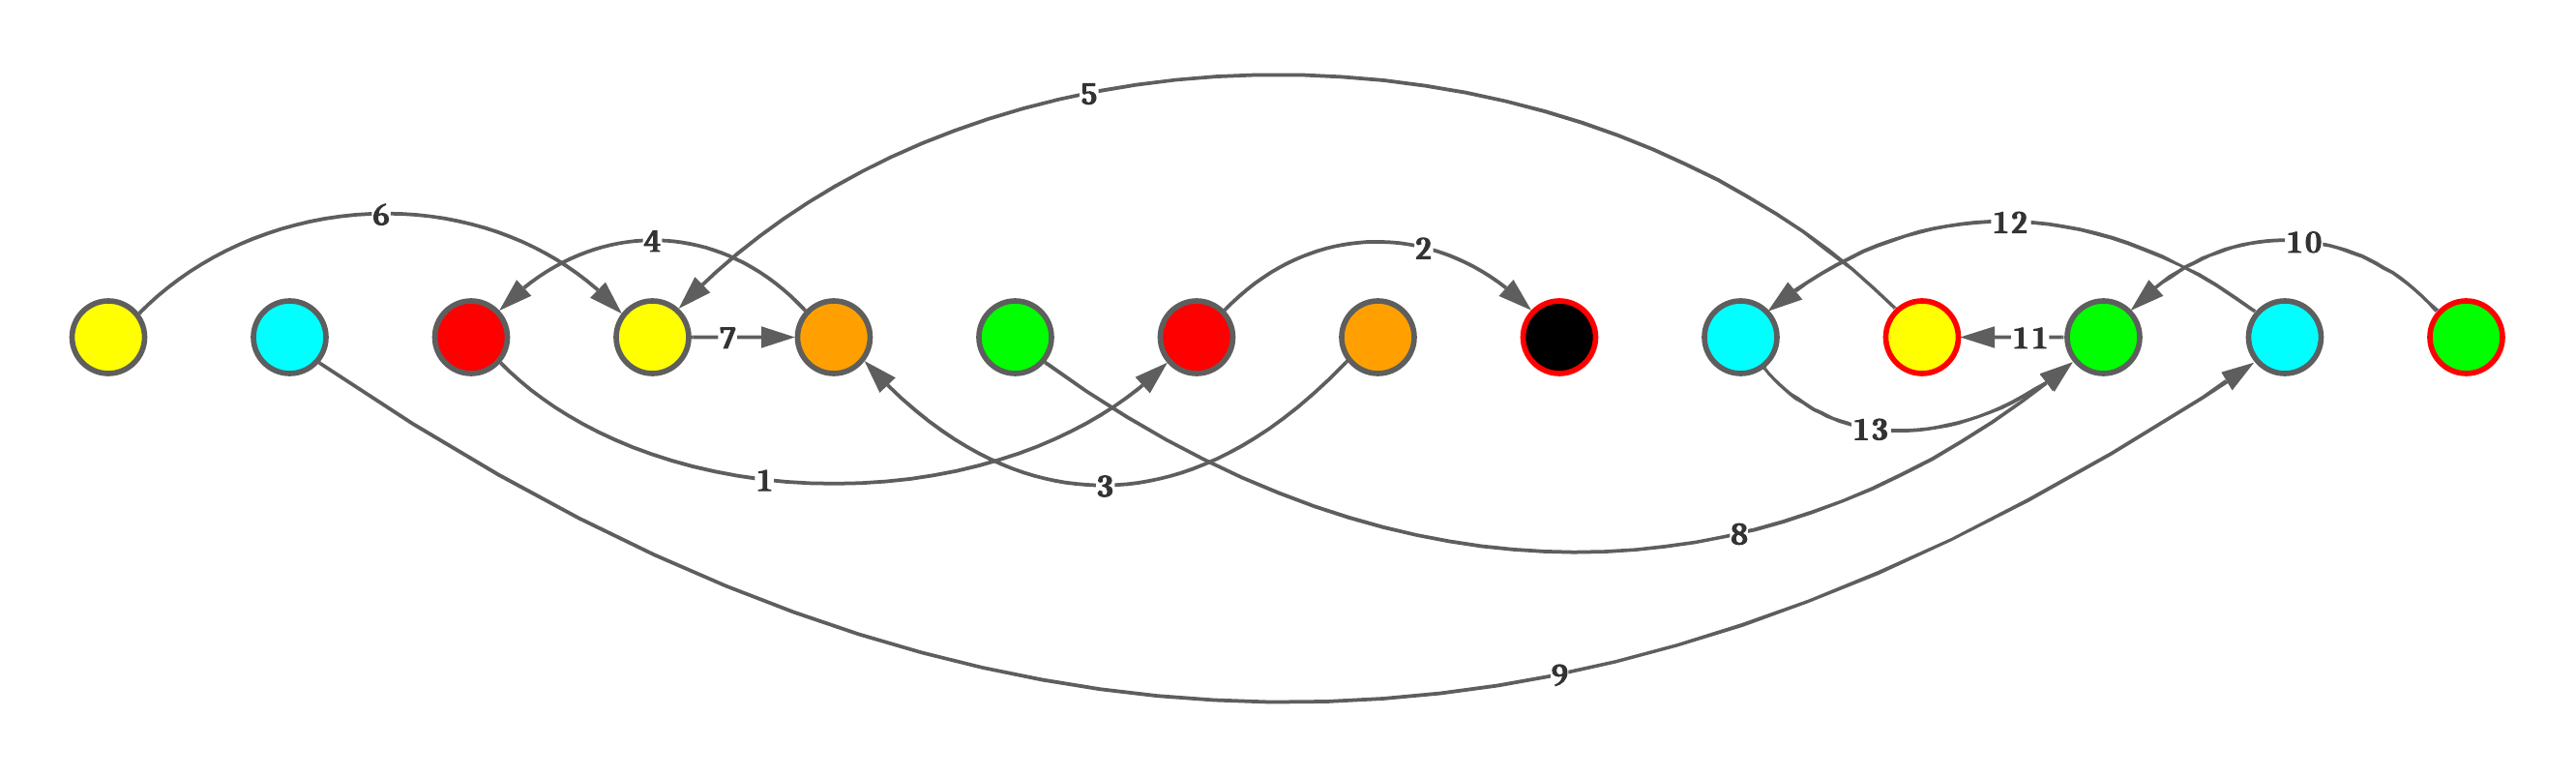
\includegraphics[width=14cm]{Images/ActSeqPic.png}
    \caption{This figure represents an activation sequence $\alpha$ with the different coloured nodes; the black, red, orange, yellow, lime and cyan nodes represent $\alpha_{\phi_0},...,\alpha_{\phi_5}$ respectively. The nodes outlined in red are the nodes contained in the sequence $(u_j)_{j=0}^k$, the function $\Gamma$ counts exactly these nodes, excluding the root node, which is the black node in this diagram.}
    \label{fig:activationsequence}
\end{figure}

We will now prove a Lemma giving a tight bound on the expected value of $\Gamma$ over random initial orderings.

\begin{lemma}\label{gamma lemma 1}
Let $\pazocal E$ be any insertion sequence of $G$, then
\[ \mathbb{E}_{\prec \in \mathcal{S}_V}[\Gamma(act(\pazocal E), \prec)] = \pazocal{O}(\log n) \]
\end{lemma}

\begin{proof}
Given some ordering $\prec$ of $V$ uniformly at random, defined by the sequence $(v_1,...,v_n)$, we can compute $\Gamma(act(\pazocal E, \prec)$ in the following way.

Create a sequence $(s_i)_{i=1}^n$ where $s_i = t$ if and only if $v_i \in \alpha_t$. Set $i_{-1}=1$. Compute $t_0 = min\{s_{t_{-1}+1},...,s_n\}$ and let $i_0=max\{i:s_i=t_0\}$. Notice that $v_{i_0} = u_0$ and $t_0 = \phi_0$. If $i_0 < n$ we can continue as follows. Compute $t_1 = min\{s_{t_{0}+1},...,s_n\}$ and let $i_1=max\{i:s_i=t_1\}$. Notice that $v_{i_1} = u_1$ and $t_1 = \phi_1$. We can continue like this forming a sequence $(i_0,...,i_k)$ until we reach $i_k = n$. We now argue that $k = \pazocal O(\log n)$.

We know that $u_0 = r$ and we expect it's position in the ordering to be $\frac{n}{2}$ since the ordering was generated uniformly at random, hence, we expect $i_0 = \frac{n}{2}$. Similarly, we expect the rightmost minimum in $\{s_{i_0+1},...,s_n\}$ to have an index of at least $i_0 + \frac{1}{2}(n - i_0)$ = $\frac{1}{2}(n+i_0)$ = $\frac{3}{4}n$, but it may be larger if there is more than one minimum. Continuing like this we can see that $\mathbb{E}[i_j] \geq n(1-2^{-1-j})$ giving us that $\mathbb{E}[i_{\log_{2}n}] \geq n-\frac{1}{2} > n - 1$ so we get that $k = \pazocal O(\log n)$.
\end{proof}

% CHAPTER 3
\section{Activation Sequences for Trees}

Fix a tree $\pazocal T=(V,E)$ with root $r$. Throughout this section we implicitly assume we are running all inputs on $\pazocal A_1$.

The activation sequences of rooted trees take a very particular form because all non-root nodes have an out-degree of exactly 1. This allows us to deduce the following Lemma, making it easy to show that the expected total recourse of $\pazocal A_1$ on trees under adversarial insertion is low.

\begin{lemma}\label{gamma lemma 2}
Let $\pazocal E$ be any insertion sequence of $\pazocal T$ and $\prec$ any initial ordering, then
\[ rec_r(\pazocal E, \prec) = \Gamma(act(\pazocal E), \prec) \]
\end{lemma}

Before proving this we must make the following simple observation.

\begin{proposition}
Let $\alpha$ be an activation sequence of $\pazocal T$. If $(x,y) \in E$, then $y$ is not activated after $x$.
\end{proposition}

\begin{proof}
Since $\pazocal T$ is a tree, there is a unique path from $x$ to $r$ and it includes $y$. Hence, when $x$ is activated (i.e. when an insertion causes $x$ to be able to reach $r$ from the first time), we know that $y$ must either be activated simultaneously or is already active.
\end{proof}

\begin{proof}[Proof of lemma 3.1]
Suppose that $rec_r(\pazocal E, \prec) > \Gamma(act(\pazocal E), \prec)$. This implies that while $x$ and $y$ are not active an edge $(x,y)$ is inserted such that $x$ is activated before $y$. Since $\pazocal T$ is a tree, $x$ can only be activated once $y$ has been activated, giving a contradiction. Hence, $rec_r(\pazocal E, \prec) \leq \Gamma(act(\pazocal E), \prec)$.

Suppose that $rec_r(\pazocal E, \prec) < \Gamma(act(\pazocal E), \prec)$. This implies that while $x$ and $y$ are not active an edge $(x,y)$ is inserted such that $y$ is activated before $x$. If such an edge is inserted, then as soon as $y$ is activated, $x$ will also be activated simultaneously, so this is not possible. Hence, $rec_r(\pazocal E, \prec) \geq \Gamma(act(\pazocal E), \prec)$.
\end{proof}

While this Lemma does not hold for DAGs in general, the second part of the proof follows from the observation we made earlier about activation sequences, so we get that $\Gamma(act(\pazocal E), \prec)$ is a lower bound on the recourse of the root for any DAG.

Now we can combine Lemma \ref{gamma lemma 1} and Lemma \ref{gamma lemma 2} to obtain the following Theorem.

\begin{theorem}
Let $\pazocal E$ be any insertion sequence of $\pazocal T$, then
\[ \mathbb{E}_{\prec \in \mathcal{S}_V}[ rec_r(\pazocal E, \prec)] = \pazocal{O}(\log n) \]
\end{theorem}

\begin{proof}
Now we can combine Lemma \ref{gamma lemma 1} and Lemma \ref{gamma lemma 2} to obtain the following equality
\[ \mathbb{E}_{\prec \in \mathcal{S}_V}[ rec_r(\pazocal E, \prec)] = \mathbb{E}_{\prec \in \mathcal{S}_V}[\Gamma(act(\pazocal E, \prec))] = \pazocal{O}(\log n) \]
\end{proof}

We can now bound the expected total recourse of $\pazocal A_1$ with a random initial ordering on trees under adversarial by $\pazocal O(n \log n)$ by applying the argument to each node individually. 

\begin{corollary}
Let $\pazocal E$ be any insertion sequence of $\pazocal T$, then
\[ \mathbb{E}_{\prec \in \mathcal{S}_V}[ rec(\pazocal E, \prec)] = \pazocal{O}(n\log n) \]
\end{corollary}

\begin{proof}
The total expected recourse is the sum of the expected recourse of every node, so by linearity of expectation we get
\[ \mathbb{E}_{\prec \in \mathcal{S}_V}[ rec(\pazocal E, \prec)] = \sum_{u \in V} \mathbb{E}_{\prec \in \mathcal{S}_V}[ rec_u(\pazocal E, \prec)] = \sum_{u \in V} \pazocal{O}(\log n) = \pazocal{O}(n\log n) \]
\end{proof}

%%%%____%%%% CHAPTER 7 : Extending the Activation Sequence Framework %%%%____%%%%

\chapter{Extending the Activation Sequence Framework}\label{chapter7}

In the previous chapter we saw that Lemma \ref{gamma lemma 2} gave us an equivalence between values of the function $\Gamma$ and the recourse of $\pazocal A_1$ trees. We also noted that this could be used to obtain a lower bound for the recourse of $\pazocal A_1$ on any DAG. One of the main result of this chapter will be an extension of this result to DAGs, allowing us fully characterize the recourse of $\pazocal A_1$ on any DAG in terms of values of $\Gamma$. Using this result we will give a reduction from Conjecture \ref{mainconjecture} to a Conjecture analogous to Lemma \ref{gamma lemma 1}.

\section{Incomplete Insertion and Activation Sequences}

Before continuing with the results in this chapter, it will be helpful to introduce some new notation to make things easier to read. Let $G=(V,E)$ be a DAG with root $r$. In Definition \ref{gammafunction}, we define a sequence of nodes, $(u_j)_{j=1}^k$, given some insertion sequence $\pazocal E$ and an ordering $\prec$, and we let $\Gamma(act(\pazocal E), \prec) = k$. If some node $u \in V$ is contained in the sequence $(u_j)_{j=1}^k$, we say that it is \textit{counted} by $\Gamma(act(\pazocal E), \prec)$. We say this in a more compact way as follows.

\begin{definition}
Given some $\pazocal E \in \mathcal S_E$, $\prec \: \in \mathcal S_V$, $u \in V$, we say that $u$ is \textbf{relevant} in $\prec$ with respect to $\pazocal E$ if $\Gamma(act(\pazocal E), \prec)$ counts $u$.
\end{definition}

In the propositions and proofs throughout with chapter, we want to be able to consider the state of the graph and the ordering after some fixed edges have been inserted, so we must extend our notation to be well defined setting. We define \textbf{incomplete insertion sequences} of $G$ to be proper subsequences of insertion sequences of $G$. We define \textbf{incomplete activation sequences} to be the activation sequences of incomplete insertion sequences. Note that the length of an incomplete activation sequence is less than $m$ and that its elements many not partition $V$. We also extend the domain of $\Gamma$ to incomplete activation sequences.

Let $\pazocal E$ and $\pazocal F$ be incomplete insertion sequences of $G$ of length $k_1$ and $k_2$ respectively such that $\{\pazocal E_i\}$ and $\{\pazocal F_i\}$ are disjoint. Let $\pazocal{EF}$ denote the potentially incomplete insertion sequence obtained by appending $\pazocal F$ to the end of $\pazocal E$. Then we denote the incomplete activation sequence of $\pazocal F$ starting after the insertion of $\pazocal E$ by $act(\pazocal E, \pazocal F)$. Note that $act(\pazocal E, \pazocal F) = (act(\pazocal{EF})_{k_1 + 1},...,act(\pazocal{EF})_{k_1 + k_2})$ and that $\Gamma(act(\pazocal E, \pazocal F), \prec) = \Gamma(act(\pazocal E\pazocal F), \prec) - \Gamma(act(\pazocal E), \prec)$.

\section{Extending Lemma \ref{gamma lemma 2} to DAGs}

Throughout this whole chapter we implicitly assume we are running all inputs on $\pazocal A_1$ and fix a DAG $G=(V,E)$ with root $r$ and initial ordering $\prec_0 \: \in \mathcal S_V$.

We now give a generalization of Lemma \ref{gamma lemma 2} that gives us an equation relating the recourse of any DAG to values of $\Gamma$. The difference between this new equation and the equation given in Lemma \ref{gamma lemma 2} is the presence of a term which is always equal to 0 when $G$ is a tree.

\begin{proposition}\label{mainobservation} Let $x^+=max(x,0)$. Given any insertion sequence $\pazocal E$ of $G$ we have that
\[ rec_r(\pazocal E, \prec_0) =  \sum_{t=1}^{m}\big(\Gamma(act(\pazocal E), \prec_{t}) - \Gamma(act(\pazocal E), \prec_{t-1})\big)^+ + \Gamma(act(\pazocal E), \prec_0) \]
\end{proposition}

Here we let $\prec_t$ denote the ordering computed by $\pazocal A_1$ after the first $t$ edges of $\pazocal E$ have been inserted. The following Lemma will be useful and allow us to give a nicer proof of this proposition.

\begin{lemma} Given any insertion sequence $\pazocal E$ of $G$ we have that
\[ \Gamma(act(\pazocal E), \prec_{t}) < \Gamma(act(\pazocal E), \prec_{t-1}) \implies \Gamma(act(\pazocal E), \prec_{t}) = \Gamma(act(\pazocal E), \prec_{t-1}) - 1  \]
\end{lemma}

\begin{proof}
Let $\pazocal U = \{u_1,...,u_k\}$ be the set of nodes relevant in $\prec_{t-1}$ with respect to $\pazocal E$. Given any $u_i,u_j \in \pazocal U$, we know that $u_i$ and $u_j$ are activated at different times. We also know that given any $u_i \in \pazocal U$ we have that $r \prec_t u_i$ if and only if $u_i$ is activated at time $t$. Now suppose that $\Gamma(act(\pazocal E), \prec_{t}) < \Gamma(act(\pazocal E), \prec_{t-1}) - 1$, then there are (at least) two nodes $u_i, u_j \in \pazocal U$ that are not relevant in $\prec_t$ with respect to $\pazocal E$, this means that both $u_i$ and $u_j$ were activated at time $t$, but $u_i$ and $u_j$ must be activated at different times, so we get a contradiction. It follows that $\Gamma(act(\pazocal E), \prec_{t}) \geq \Gamma(act(\pazocal E), \prec_{t-1}) - 1$, so we have that $\Gamma(act(\pazocal E), \prec_{t}) = \Gamma(act(\pazocal E), \prec_{t-1}) - 1$.
\end{proof}

\begin{proof}[\textbf{Proof of Proposition \ref{mainobservation}}]
Fix some $\pazocal E \in \mathcal S_E$. By the construction of $\Gamma$, after the insertion of the edge $\pazocal E_{t-1}$, we have that $\Gamma(act(\pazocal E), \prec_{t}) < \Gamma(act(\pazocal E), \prec_{t-1})$ if and only if $r$ is moved during the insertion of $\pazocal E_{t-1}$. By Lemma 1, this tells us that
\[ rec_r(\pazocal E, \prec_{0})_t = 1 \iff \Gamma(act(\pazocal E), \prec_{t}) = \Gamma(act(\pazocal E), \prec_{t-1}) - 1 \]
So we can form the equation
\[ rec_r(\pazocal E, \prec_0) =  \sum_{t=1}^{m}\big(\Gamma(act(\pazocal E), \prec_{t-1}) - \Gamma(act(\pazocal E), \prec_{t})\big)^+ \]
Since the expression on the right hand side counts the total amount that $\Gamma(act(\pazocal E), \prec_{t})$ \textit{decreases} as we increase $t$ from $1$ to $m$, and we know that $\Gamma(act(\pazocal E), \prec_{m}) = 0$, we can see that this is equal to the starting value $\Gamma(act(\pazocal E), \prec_0)$ plus the total amount that $\Gamma(act(\pazocal E), \prec_{t})$ \textit{increases} as we increase $t$ from $1$ to $m$. Hence, we get that
\[ rec_r(\pazocal E, \prec_0) =  \sum_{t=1}^{m}\big(\Gamma(act(\pazocal E), \prec_{t}) - \Gamma(act(\pazocal E), \prec_{t-1})\big)^+ + \Gamma(act(\pazocal E), \prec_0) \]
\end{proof}

\section{$\Gamma$ Under Random-Order Arrival}

I will now introduce a new conjecture about the values taken by $\Gamma$ under random order arrival with respect to some fixed ordering. I will then show that this conjecture implies Conjecture \ref{mainconjecture}.

\begin{conjecture}\label{finallemma}
Let $F \subseteq E$, $\pazocal E \in \mathcal S_{E \setminus F}$, $\prec \: \in \mathcal S_V$, then we have that
\[ \mathbb E_{\pazocal F \in \mathcal S_F}[\Gamma(act(\pazocal E, \pazocal F), \prec)] = \polylog{\vert F \vert} \]
\end{conjecture}

For the rest of this chapter, any lemma or theorem marked with an asterisk follows from assuming that Conjecture \ref{finallemma} is true. Technically this means they aren't actually lemmas or theorems, but this is more elegant than labelling them all conjectures.

\begin{lemma*}\label{gamma analog}
Given any $\prec \: \in \mathcal S_V$ we have that
\[ \mathbb E_{\pazocal E \in \mathcal S_E}[\Gamma(act(\pazocal E), \prec)] = \polylog n \]
\end{lemma*}

\begin{proof}
Follows directly from conjecture \ref{finallemma} by setting $F=E$.
\end{proof}

We can see that lemma* \ref{gamma analog} is analogous to lemma \ref{gamma lemma 2}, the only relevant difference is that here we are fixing the ordering and taking expectation of insertion sequences instead of fixing the insertion sequence and taking expectation over orderings.



% \begin{lemma}[\color{red}{UNPROVEN}\color{black}]
% Let $\{E_1,...,E_k\}$ be any partition of $E$. Let $\pazocal S \in [k]^m$ be any sequence containing exactly $\vert E_i \vert$ many $i$ for each $i \in [k]$. We call such a sequence an \textbf{instruction sequence} for $\{E_1,...,E_k\}$. We say that $\pazocal E \in \mathcal S_E$ agrees with $\pazocal S$ if we have that for all $i \in [m]$, $\pazocal E_i \in E_{\pazocal S_i}$. Given any $\prec \: \in \mathcal S_V$ we have that
% \[ \mathbb E_{\pazocal F \in \mathcal S_{E_2}}[\Gamma(act(\pazocal E \pazocal F), \prec) - \Gamma(act(\pazocal E), \prec)] = \polylog{\vert E_2 \vert} \]
% \end{lemma}

We now define some useful functions that will make the notation easier to read.

\begin{definition}
Let $\pazocal E \in \mathcal S_E$, $t \in [m]$, we define the following functions.

\begin{enumerate}
    \item Let $\chi_t(\pazocal E, \prec_0)$ be the indicator function for the event that $\Gamma(act(\pazocal E), \prec_{t}) > \Gamma(act(\pazocal E), \prec_{t-1})$
    \item Let $\lambda_t(\pazocal E, \prec_0)$ be the indicator function for the event that $\pazocal E_{t}=(u,v)$ where $u$ is relevant in $\prec_{t-1}$ with respect to $\pazocal E$
    \item Let $\Lambda_t(\pazocal E, \prec_0) = \big(\Gamma(act(\pazocal E), \prec_{t}) - \Gamma(act(\pazocal E), \prec_{t-1})\big)^+$
\end{enumerate}

\end{definition}

\begin{proposition}
Given any potentially incomplete insertion sequence $\pazocal E$ of $G$ of length $t$, we have that
\[ \Gamma(act(\pazocal E),\prec_t) = 0 \]
\end{proposition}

\begin{proof}
Suppose that $\Gamma(act(\pazocal E),\prec_t) > 0$, then some node $u$ is relevant in $\prec_t$ with respect to $\pazocal E$. This implies that $r \prec_t u$ and that for some $i \leq t$ the insertion of $\pazocal E_i$ causes $u$ to be activated, but after $u$ is activated we know that it must appear before $r$ in the ordering, in other words, for all $j \geq i$ we have $u \prec_j r$. But this tells us that $u \prec_t r$, giving us a contradiction.
\end{proof}

\begin{proposition}\label{chileqlam}
Let $\pazocal E \in \mathcal S_E$, $t \in [m]$, then \[\chi_t(\pazocal E, \prec_0) \leq \lambda_t(\pazocal E, \prec_0)\]
\end{proposition}

\begin{proof}
Suppose that $\lambda_t(\pazocal E, \prec_0)=1$, i.e. that $\Gamma(act(\pazocal E), \prec_{t}) > \Gamma(act(\pazocal E), \prec_{t-1})$. Then the insertion of $\pazocal E_t = (u,v)$ causes some node $w$ which is relevant in $\prec_t$ but not in $\prec_{t-1}$ to incur recourse. Since $w \in reach_t(u)$ and neither are active at time $t$, we get that $u$ is not activated after $w$, so since $w$ is relevant in $\prec_t$ we get that $u$ is relevant in $\prec_{t-1}$, i.e. that $\lambda_t(\pazocal E, \prec_0) = 1$. Hence, $\chi_t(\pazocal E, \prec_0) \leq \lambda_t(\pazocal E, \prec_0)$.
\end{proof}

We now give two lemmas* use them to prove that conjecture \ref{finallemma} implies conjecture \ref{mainconjecture}. We will use a proposition given by Bernstein et al. in \cite{BernsteinC18} which allows us to assume that the maximum degree of any node in the graph is $\pazocal O(m/n)$. So we assume that the maximum degree of any node in $G$ is $\Delta = \pazocal O(m/n)$.

\begin{lemma*}\label{first reduction lemma}
Let $F \subseteq E$, $\pazocal E = (\pazocal E_1,...,\pazocal E_{t-1}) \in \mathcal S_{E \setminus F}$, then we have that
\[ \mathbb E_{\pazocal F \in \mathcal S_F} [\lambda_t(\pazocal E \pazocal F, \prec_0)] \leq \frac{\Delta\polylog n}{m-t+1} \]
\end{lemma*}

\begin{lemma*}\label{second reduction lemma} 
Let $F \subseteq E$, $\pazocal E = (\pazocal E_1,...,\pazocal E_{t-1}) \in \mathcal S_{E \setminus F}$, then we have that
\[ \mathbb E_{\pazocal F \in \mathcal S_F} [\Lambda_t(\pazocal E \pazocal F, \prec_0) \vert \lambda_t(\pazocal E \pazocal F, \prec_0) = 1] = \polylog n\]
\end{lemma*}

\begin{theorem*}\label{second reduction lemma} 
$\mathbb E_{\pazocal E \in \mathcal S_E}[rec(\pazocal E, \prec_0)] = \tilde{\pazocal O}(m)$
\end{theorem*}

\begin{proof}
We can see that Lemma* \ref{first reduction lemma} implies that
\[ \mathbb E_{\pazocal E \in \mathcal S_E}[\lambda_t(\pazocal E, \prec_0)] \leq \frac{\Delta\polylog n}{m-t+1} \]
and that Lemma* \ref{second reduction lemma} implies that
\[ \mathbb E_{\pazocal E \in \mathcal S_E}[\Lambda_t(\pazocal E, \prec_0) \vert \lambda_t(\pazocal E, \prec_0) = 1] = \polylog n\]

Since $\chi_t = 0$ if and only if $\Lambda_t = 0$, and $\chi_t \leq \lambda_t$ by Proposition \ref{chileqlam}, we can see that $\mathbb E_{\pazocal E \in \mathcal S_E}[\Lambda_t(\pazocal E, \prec_0) \vert \lambda_t(\pazocal E, \prec_0) = 0] = 0$. Applying the law of total expectation we get that

\[ \mathbb E_{\pazocal E \in \mathcal S_E} [\Lambda_t(\pazocal E, \prec_0)]  = \mathbb E_{\pazocal E} [\Lambda_t(\pazocal E, \prec_0) \vert \lambda_t(\pazocal E, \prec_0) = 1] \cdot \mathbb P [\lambda_t(\pazocal E, \prec_0) = 1] \]

\[ \leq \mathbb E_{\pazocal E} [\Lambda_t(\pazocal E, \prec_0) \vert \lambda_t(\pazocal E, \prec_0) = 1] \cdot \frac{\Delta\polylog n}{m-t+1} = \frac{\Delta\polylog n}{m-t+1} \]

We can now take expectations over insertion sequences on both sides of the equation in Proposition \ref{mainobservation} to obtain
\[ \mathbb E_{\pazocal E \in \mathcal S_E}[rec_r(\pazocal E, \prec_0)] =  \sum_{t=1}^{m} \mathbb E_{\pazocal E \in \mathcal S_E}[ \Lambda_t(\pazocal E, \prec_0) ] + \mathbb E_{\pazocal E \in \mathcal S_E}[\Gamma(act(\pazocal E), \prec_0)] \]
\[ \leq \sum_{t=1}^{m} \frac{\Delta\polylog n}{m-t+1} + \polylog n = \Delta \polylog n \]

So it follows that
\[ \mathbb E_{\pazocal E \in \mathcal S_E}[rec(\pazocal E, \prec_0)] = \sum_{x \in V} \mathbb E_{\pazocal E \in \mathcal S_E}[rec_x(\pazocal E, \prec_0)] = \sum_{x \in V} \Delta \polylog n = \tilde{\pazocal O}(m) \]
\end{proof}

\subsection{Proof of Lemma* \ref{first reduction lemma}}

\begin{proof}
Let $V=\{x_1,...,x_n\}$. By Lemma 3 we can see that
\[ \mathbb E_{\pazocal F \in \mathcal S_F}[\Gamma(act(\pazocal E \pazocal F), \prec_{t-1})] = \mathbb E_{\pazocal F \in \mathcal S_F}[\Gamma(act(\pazocal E \pazocal F), \prec_{t-1}) - \Gamma(act(\pazocal E), \prec_{t-1})] = \polylog n \] 
Suppose the rest of the edges are inserted uniformly at random. Let $p(x_i)$ be the probability that $x_i$ is relevant in $\prec_{t-1}$. We can see that
\[ p(x_1) +...+p(x_n) =  \mathbb E_{\pazocal F \in \mathcal S_F}[\Gamma(act(\pazocal E \pazocal F), \prec_{t-1})] = \polylog n \]
Since $\pazocal E_t=(u,v)$ is equally likely to be any of the edges in $F$ and each node has at most $\Delta$ outgoing edges, we get that
\[ \mathbb E_{\pazocal F}[\lambda_t(\pazocal E \pazocal F, \prec_0)] = p(x_1) \cdot \mathbb P[u=x_1]+...+ p(x_n) \cdot \mathbb P[u=x_n]\]
\[ \leq p(x_1) \cdot \frac{\Delta}{m-t+1}+...+ p(x_n) \cdot \frac{\Delta}{m-t+1} =\frac{\Delta\polylog n}{m-t+1}\]
\end{proof}

\subsection{Proof of Lemma* \ref{second reduction lemma}}

\subsubsection{Outline}

Suppose we have inserted the incomplete insertion sequence $\pazocal E = (\pazocal E_1,...,\pazocal E_{t-1})$ into the graph and let $F=E \setminus \{\pazocal E_t\}$. In this context, given some $\pazocal F \in \mathcal S_F$ let $\overline{\pazocal F}$ denote $\pazocal{EF}$ and assume that $t \leq m$. Let $S \subseteq \mathcal S_F$ be the set of incomplete insertion sequences $\pazocal F$ such that $\overline{\pazocal F}_t=(u,v)$ where $u$ is relevant in $\prec_{t-1}$, in other words, such that $\lambda_t(\overline{\pazocal F}, \prec_0)=1$. We assume that $\Lambda_t \geq 0$. Let $f \in F$, then let $S_f \subseteq S$ be the set of all $\pazocal F \in S$ such that $\overline{\pazocal F}_t = f$. Note that $S_f$ may be empty and that $\{ S_f \}_{f \in F}$ is a partition of $S$. The idea of this proof is to define an equivalence relation, $\simeq$, on $S_f$ (and hence on $S$) such that, given any $f \in F$, for any $\pazocal F^\star \in S_f$ we have
\[ \mathbb E_{\pazocal F \in [\pazocal F^\star]_{\simeq}}[\Lambda_t(\overline{\pazocal F}, \prec_0)] = \polylog n \]

Notice crucially that this expression requires $\prec_t$ to be defined, which is why we start by restricting to $S_f$. Once we have established this, we can construct a partition $P_1,...,P_k$ of $S$ such that for all $i \in [k]$ we have $\mathbb E_{\pazocal F \in P_i}[\Lambda_t(\overline{\pazocal F}, \prec_0)] = \polylog n$ and it will follow that
\[ \mathbb E_{\pazocal F \in \mathcal S_F} [\Lambda_t(\pazocal E \pazocal F, \prec_0) \vert \lambda_t(\pazocal E \pazocal F, \prec_0) = 1] = \mathbb E_{\pazocal F \in S} [\Lambda_t(\overline{\pazocal F}, \prec_0)]= \polylog n \]

\subsubsection{Proof}

\begin{proof}

We start off by defining $\simeq$ and proving that it defines an equivalence relation. Fix some $f \in F$ and let $\prec_t \sim (y_1,...,y_{l_1},x_1,...,x_k,y_{l_1+1},...,y_{l_2})$ where the startpoint of $f$ is $x_1$ and $x_2,...,x_k$ are the nodes that incur a recourse during the insertion of $f$.

Given some $\pazocal F \in S_f$, we define $\tau_1(\pazocal F)$ to the number $i \in [m]$ such that $\overline{\pazocal F}_i$ is the first insertion that causes a node in $\{x_1\}_{j=1}^{k}$ to be activated. Similarly, we define $\tau_2(\pazocal F)$ to the number $i \in [m]$ such that $\overline{\pazocal F}_i$ is the first insertion that causes a node in $\{y_j\}_{j=l_1+1}^{l_2}$ to be activated. Since $x_1$ is relevant in $\prec_{t-1}$, and if $x_j$ is active at time $s \geq t$ then $x_1$ is too, it follows that $\tau_1(\pazocal F) < \tau_2(\pazocal F)$.

\begin{definition}
Let $f \in F$ and $\pazocal F, \pazocal F^\star \in S_f$. We say that $\pazocal F \simeq \pazocal F^\star$ if the following hold.

\begin{enumerate}
    \item $\tau_1(\pazocal F) = \tau_1(\pazocal F^\star)$ and $\tau_2(\pazocal F) = \tau_2(\pazocal F^\star)$
    \item $\pazocal F^\star$ can be obtained by starting with $\pazocal F$ and permuting the positions of the edges in $\pazocal F$ that appear strictly between the edges $\overline{\pazocal F}_i$ and $\overline{\pazocal F}_j$ with $i=\tau_1(\pazocal F)$ and $j=\tau_2(\pazocal F)$.
\end{enumerate}
\end{definition}

The fact that permuting edges as described doesn't change the value of $\tau_1(\pazocal F)$ or $\tau_2(\pazocal F)$ can be used to show that $\simeq$ is an equivalence relation on $S_f$. This can be proven using the \textit{memoryless} property of activation sequences, in other words, the fact that the activation sequence after some point only depends on the order in which the remaining edges will be inserted and does not depend on the order in which the edges already in the graph were inserted.

Let $\pazocal F \in S_f$ and let $i=\tau_1(\pazocal F)$ and $j=\tau_2(\pazocal F)$. An important observation is that any node $y \in \{y_i\}_{i=1}^{l_2}$ is relevant in $\prec_{t-1}$ if and only it is relevant in $\prec_t$ with respect to $\overline{\pazocal F}$. This tells us that $\Lambda_t$ is the difference in the number of nodes from $\{x_i\}$ relevant in $\prec_t$ and $\prec_{t-1}$. This difference can only be created by the edged contained strictly between $\overline{\pazocal F}_i$ and $\overline{\pazocal F}_j$. Let $\overline{\pazocal F}^1 = (\overline{\pazocal F}_1,...,\overline{\pazocal F}_i)$, $\overline{\pazocal F}^2 = (\overline{\pazocal F}_{i+1},...,\overline{\pazocal F}_{j-1})$ and $\overline{\pazocal F}^3 = (\overline{\pazocal F}_{j+1},...,\overline{\pazocal F}_m)$. Then we have that

\[ \Lambda_t(\overline{\pazocal F}, \prec_0) = \Gamma(act(\overline{\pazocal F}), \prec_{t}) - \Gamma(act(\overline{\pazocal F}), \prec_{t-1}) \]
\[ =\big(\Gamma(act(\overline{\pazocal F}^1), \prec_{t}) + \Gamma(act(\overline{\pazocal F}^1, \overline{\pazocal F}^2), \prec_{t}) + \Gamma(act(\overline{\pazocal F}^1\overline{\pazocal F}^2, \overline{\pazocal F}^3), \prec_{t}) \big) \]
\[ - \big(\Gamma(act(\overline{\pazocal F}^1), \prec_{t-1}) + \Gamma(act(\overline{\pazocal F}^1, \overline{\pazocal F}^2), \prec_{t-1}) + \Gamma(act(\overline{\pazocal F}^1\overline{\pazocal F}^2, \overline{\pazocal F}^3), \prec_{t-1}) \big)\]
\[ = \Gamma(act(\overline{\pazocal F}^1, \overline{\pazocal F}^2), \prec_{t}) - \Gamma(act(\overline{\pazocal F}^1, \overline{\pazocal F}^2), \prec_{t-1}) \leq \Gamma(act(\overline{\pazocal F}^1, \overline{\pazocal F}^2), \prec_{t}) \]

Let $\pazocal F^\star \in S_f$ and let $P=[\pazocal F^\star]_{\simeq}$. Given any $\pazocal F \in P$, $\overline{\pazocal F}^1 = (\overline{\pazocal F}^\star)^1$. So we get that $ \mathbb E_{\pazocal F \in P} [\Gamma(act(\overline{\pazocal F}^1, \overline{\pazocal F}^2), \prec_{t})] = \polylog n$ by Lemma 3. This is because $\overline{\pazocal F}^1$ is a fixed incomplete insertion sequence for all $\pazocal F \in P$, and because the (multi) set of incomplete insertion sequences $\overline{\pazocal F}^2$ corresponding to $\pazocal F \in P$ is exactly all incomplete insertion sequences over the edges contained in $(\overline{\pazocal F}^\star)^2$.
\[ \mathbb E_{\pazocal F \in P} [\Lambda_t(\overline{\pazocal F}, \prec_0)] \leq \mathbb E_{\pazocal F \in P} [\Gamma(act(\overline{\pazocal F}^1, \overline{\pazocal F}^2), \prec_{t})] = \polylog n \]
\end{proof}

%%%%____%%%% BIBLIOGRAPHY %%%%____%%%%

\bibliographystyle{alpha}
\bibliography{refs.bib}

\end{document}